% !TEX root = main.tex
\section{Formalism}

\subsection{Decay rates and \CP-observables}

%We define the purely hadronic amplitudes for a given phasespace point $x$.
%The weak phase dependence is written latter explicitly in the pdf.

%\begin{align}
%	A(B_s^0 \to D_s^{-} K^{+} \pi\pi) &\equiv A(x) = \sum_i a_i \, A_i(x)   \\
%	A(\bar B_s^0 \to D_s^{-} K^{+} \pi\pi) &\equiv \bar A(x) = \sum_i \bar a_i \,\bar A_i(x)   \\
%	A(\bar B_s^0 \to D_s^{+} K^{-} \pi\pi) &= A(x)  \, \, \text{(Assuming no direct CPV)} \\
%	A(B_s^0 \to D_s^{+} K^{-} \pi\pi) &= \bar A(x)  \, \, \text{(Assuming no direct CPV)} 
%\end{align}



%\begin{align}
%	A(B_s^0 \to D_s^{-} K^{+} \pi\pi) &\equiv A(x) = \sum_i a_i \, A_i(x)   \\
%	A(B_s^0 \to D_s^{+} K^{-} \pi\pi) &\equiv \bar A(\bar x) = \sum_i \bar a_i \,\bar A_i(\bar x)    \\
%	A(\bar B_s^0 \to D_s^{-} K^{+} \pi\pi) &= \bar A(x)  \, \, \text{(Assuming no direct CPV)} \\
%	A(\bar B_s^0 \to D_s^{+} K^{-} \pi\pi) &= A(\bar x)  \, \, \text{(Assuming no direct CPV)} 
%\end{align}

%The full time-dependent amplitude pdf is given by:

The differential decay rate of $B_s^{0}$ or $\bar B_s^{0}$ decays to the final state $D_s^{-} K^{+} \pi\pi$ or $D_s^{+} K^{-} \pi\pi$
is given by: 
\begin{equation}
\begin{split}
\label{eq:PDF_full}
%	P(x,t,q_t,q_f) &\propto  [
	\frac{ \text{d}\Gamma(\phsPoint,t,q_t,q_f)}{ e^{- \Gamma_s t} \, \text{d}t \, \text{d}\Phi_4} &\propto  
	 \left( \vert \mathcal A^c_{f}(\phsPoint) \vert^2 + \vert \mathcal A^u_{f}(\phsPoint) \vert^2 \right) \, \text{cosh} \left( \frac{\Delta \Gamma_s \, t}{2}\right) \\
	 & + q_t \, q_f \,  \left( \vert \mathcal A^c_{f}(\phsPoint) \vert^2 - \vert \mathcal A^u_{f}(\phsPoint)  \vert^2 \right) \, \text{cos} \left(\Delta m_s \, t \right)  \\
	 & -2 \text{Re}\left( \mathcal A^c_{f}(\phsPoint)^{*}  \, \mathcal A^u_{f}(\phsPoint)  \, e^{-i q_f (\gamma - 2\beta_s)}  \right) \, \text{sinh} \left( \frac{\Delta \Gamma_s \, t}{2}\right)  \\
	 & -2 \, q_t \, q_f \, \text{Im}\left( \mathcal A^c_{f}(\phsPoint)^{*} \, \mathcal A^u_{f}(\phsPoint)  \, e^{-i q_f (\gamma - 2\beta_s)}  \right)\, \text{sin} \left(\Delta m_s \, t \right)  
\end{split}
\end{equation}
where $q_t = +1$ (-1) refers to an initially produced $B_s^{0}$ ($\bar B_s^{0}$) flavour eigenstate, $q_t = 0$ to an undetermined initial flavour,
$q_f$ = +1  or -1 denotes $f = D_s^{-} K^{+} \pi\pi$ or $\bar f = D_s^{+} K^{-} \pi\pi$ final states
and $\Gamma_s$, $\Delta \Gamma_s$ and $\Delta m_s$ are 
the width average, the width difference 
and the mass difference of the two $B_s$ 
mass eigenstates.
%We choose a convention in which $\Delta\Gamma_s = \Gamma_L - \Gamma_H < 0$ and $\Delta m_s = m_H - m_L > 0$, where the indices $H$ and $L$ refer to the heavy and light mass eigenstates of the $B_s$ meson.
We choose a convention in which $\Delta\Gamma_s < 0$ and $\Delta m_s > 0$. 
We further assume $\vert q/p \vert = 1$ for the complex coefficients $p$ and $q$ which relate the $B_s$ meson mass eigenstates to the flavour eigenstates (no \CP violation
in the mixing).
The CKM angle $\gamma$ can be extracted from the \CP violating phase associated to the interference between mixing and decay, $\gamma - 2 \beta_s $, 
since the $B_s^{0}-\bar B_s^{0}$ mixing phase, $\beta_s$, is well constrained from $B_s \to J/\psi \, \phi$ and related modes. 

The static total decay amplitudes  $\mathcal A^c_{f}(\phsPoint)$  and $ \mathcal A^u_{f}(\phsPoint)$ 
are given by the coherent sum over all intermediate state amplitudes $A_i(\phsPoint)$, each weighted by a complex coefficient
describing the relative magnitude and phase
which is to be determined from data,
 \begin{align}
 \mathcal A(B_s^0 \to D_s^{-} K^{+} \pi\pi) &\equiv \mathcal{A}^c_f(\phsPoint) = \sum_i a^c_i \, A_i(\phsPoint)   \\
 \mathcal A(\bar B_s^0 \to D_s^{-} K^{+} \pi\pi) &\equiv \mathcal A^u_f(\phsPoint)  =  \sum_i  a^u_i \, A_i(\phsPoint)   
% \\
 \end{align}
where the superscript $c$ ($u$) indicates a $b \to c$ ($b\to u$) quark-level transition  
and $\phsPoint$ 
represents a unique set of kinematic conditions within the five-dimensional phase space of the decay.
%Each final state particle contributes three observables,
%manifesting in their three-momentum,
%summing up to twelve observables in total.
%%Out of them, four are redundant due to
%Four of them are redundant 
%due to four-momentum conservation and
%%since only spin-0 particles are involved, 
%%there is no preferred direction in space  
%the overall orientation of the system can be integrated out.
%The remaining  five independent degrees of freedom unambiguously determine the kinematics of the decay.
Convenient choices for the kinematic observables
include the invariant mass combinations of the final state particles %, with four-momenta $p_{i}$,
%\begin{align}
%	\nonumber
%	m^{2}_{ij} &= (p_{i}+p_{j})^{2} , \\
%	m^{2}_{ijk} &= (p_{i}+p_{j}+p_{k})^{2} \, 
%\end{align}
or acoplanarity and helicity angles. % \cite{Beneke:2006hg,Aaij:2015kba}.
%It is however important
%to take into account that, while $m^2_{12}, m^2_{23}$ are sufficient
%to fully describe a three-body decay, the obvious extension to
%four-body decays with $m^{2}_{ij}, m^{2}_{ijk}$ requires additional
%care, as these variables alone are insufficient to describe the parity-odd
%moments possible in four-body kinematics.
In practice, we do not need to choose a particular five-dimensional
basis, but use the full four-vectors of the decay in our
analysis. 
The dimensionality is handled by the phase space element which can be written in terms of any set of five independent kinematic observables, $\phsPoint = (x_1, \ldots, x_5)$, as
\begin{equation}
	\dphs = \phsd(\phsPoint) \, \dphsPoint ,
\end{equation}
where $\phi_{4}(\phsPoint ) = \left\vert  \frac{\partial \phs}{\partial(x_1, \ldots x_5)} \right\vert$ is the phase space density.
In contrast to three-body decays, the four-body phase space density
function is not flat in the usual kinematic variables.  
An analytic expression for \phsd\ can be found
in Ref.~\cite{kinematics}, but is not needed in practice, see Sec.~\ref{sec:phasespaceAcceptance}.

\clearpage
Assuming there is no direct \CP violation in the $B_s$ decay implies for the $\CP$ conjugate transition amplitudes:
\begin{align}
\mathcal A(\bar B_s^0 \to \bar f) &=  \mathcal A^c_{\bar f}(\phsPoint) = \mathcal A^c_f(\phsPointCP)  \\       
\mathcal A(B_s^0 \to \bar f) &= \mathcal A^u_{\bar f}(\phsPoint)  = \mathcal A^u_{f}(\phsPointCP) 
\end{align}
where the \CP-conjugate phase space point $\phsPointCP$ is defined such that it is mapped onto $\phsPoint$ by the interchange of final state charges, and the reversal of three-momenta.
%If $\phsPoint$, $\phsPointCP$ are expressed as a function of the
%four-momenta $(E_i, \vec{p}_i)$ (where $i$ labels the particle), this
%implies for \prt{\Dz \to K^+ K^- \pi^+ \pi^-} that
%\begin{align}
%\lefteqn{\phsPointCP\left[ (E_{K^+}, \vec{p}_{K^+}), (E_{K^-}, \vec{p}_{K^-}), (E_{\pi^+}, \vec{p}_{\pi^+}), (E_{\pi^-}, \vec{p}_{\pi^-})\right]} & \nonumber \\
% &\equiv
%\phsPoint\left[ (E_{K^-}, -\vec{p}_{K^-}), (E_{K^+}, -\vec{p}_{K^+}), (E_{\pi^-}, -\vec{p}_{\pi^-}), (E_{\pi^+}, -\vec{p}_{\pi^+})\right],
%\end{align} 
%and equivalently for \prt{\Dz \to \pi^+\pi^-\pi^+\pi^-}. 
The phenomenological description of the intermediate state amplitudes is discussed in Sec.~\ref{ssec:ampModel}.
\\

Rather than developing an amplitude model describing the whole phase space,
it is also possible to determine the CKM angle $\gamma$, in a model-independent way, from the decay-time distribution only.
The differential decay rate  integrated over the phase space yields:
\begin{align}
\label{eq:PDF_intX}
	\nonumber
	\int \frac{\text{d}\Gamma(x,t,q_t,q_f)}{e^{- \Gamma_s t} \, \text{d}t \,  \text{d}\Phi_4}  \, \text{d}\Phi_4 &\propto    
	\, \text{cosh} \left( \frac{\Delta \Gamma_s \, t}{2}\right) 
	  + q_t \, q_f \, C \, \text{cos} \left( \Delta m_s \, t \right)   \\
	 & +  D_{f} \, \text{sinh} \left( \frac{\Delta \Gamma_s \, t}{2}\right)  
	  - q_t  \, S_{f}\, \text{sin} \left(\Delta m_s \, t \right)  
\end{align}
where the same convention for the \CP coefficients as for the $B_s \to D_s K$ analysis is used:
\begin{align}
\label{eq:CPcoeff}
	C= & \frac{1-r^2}{1+r^2}   \\
	D_{f} = &  -\frac{2 \, r \, \kappa \, \text{cos}\left(\delta-q_f \, (\gamma-2\beta_s)\right)}{1+r^2}   \\
	S_{f} = & \,  q_f \, \frac{2 \, r \, \kappa \, \text{sin}\left(\delta-q_f \, (\gamma-2\beta_s)\right)}{1+r^2}   
\end{align}
The coherence factor $\kappa$, the strong phase difference $\delta$ and the ratio of the suppressed ($b\to u$) over favored ($b\to c$) decay mode, averaged over the 
phase space, are defined as:
\begin{align}
\label{eq:coherenceFactor}
	\kappa \, e^{i\delta} &\equiv \, \frac{\int \mathcal A^c_f(x)^{*} \, \mathcal A^u_f(x)  \, \dphs}{\sqrt{\int \vert \mathcal A^c_f(x) \vert^2 \, \dphs} \sqrt{\int \vert \mathcal A^u_f(x) \vert^2 \, \dphs}  } \\
	r &\equiv \, \frac{\sqrt{\int \vert \mathcal A^u_f(x)\vert^2 \, \dphs }}{\sqrt{\int \vert \mathcal A^c_f(x)\vert^2 \, \dphs}} .
\end{align}
The five \CP coefficients $C,D\equiv D_f,\bar D \equiv D_{\bar{f}},S \equiv S_f,\bar S \equiv S_{\bar{f}}$
can be extracted from a fit to the decay-time distribution
which allows to infer the four physical observables $r,\delta,\gamma,\kappa$ 
as discussed in more detail in Sect.~\ref{sec:validation}.
This approach will be called phase-space integrated fit in the following.
In contrast, the approach using Eq.~\ref{eq:PDF_full} will be referred to as full time-dependent amplitude fit. 
In case of the phase-space integrated fit, 
the coherence factor dilutes the sensitivity to the weak phase $\gamma$ due to the integration over the interfering amplitudes across the phase space.
The value of $\kappa$ is bounded between zero and unity.
The latter corresponds to the limit of only one contributing intermediate state in which case the same sensitivity as in $B_s \to D_s K$ decays is reached, 
while $\kappa = 0$ would result in no sensitivity to $\gamma$ at all.

\clearpage
\subsection{Amplitude model}
\label{ssec:ampModel}

To construct the intermediate state amplitudes $A_{i}(\phsPoint )$,
the isobar approach is used, which 
assumes that
the decay process can be factorized into subsequent two-body decay amplitudes \cite{isobar1,isobar,isobar2}.
This gives rise to two different decay topologies;
quasi two-body decays
$B_s \to (R_{1} \to h_{1}\,h_{2}) \, (R_{2} \to h_{3}\,h_{4})$ 
or cascade decays
$B_s \to h_{1} \, \left[R_{1} \to h_{2} \,  (R_{2} \to h_{3} \, h_{4}) \right]$.
In either case, the intermediate state amplitude is parameterized as a product of
orbital angular momentum, $L$, dependent 
form factors $B_{L}$, included for each vertex of the decay tree, 
Breit-Wigner propagators $T_{R}$,  included for each resonance $R$,
and an overall angular distribution represented by a spin factor $S$,
\begin{equation}
	A_{i}(\phsPoint ) =  B_{L_{B_s}}(\bold x) \, [B_{L_{R_{1}}}(\phsPoint )  \, T_{R_{1}}(\phsPoint )] \, [B_{L_{R_{2}}}(\phsPoint ) \, T_{R_{2}}(\phsPoint )]  \,  S_{i}(\phsPoint )  \, .
	\label{eq:amp4}
\end{equation}

The following description of the individual components is adapted from Ref.~\cite{dArgent:2017gzv} 
and only included for completeness.

%\clearpage
\subsubsection{Form Factors and Resonance Lineshapes}
\label{ssec:lineshapes}

To account for the finite size of the decaying resonances,
the Blatt-Weisskopf penetration factors, 
derived in Ref.~\cite{Bl2}
by assuming a square well interaction potential with radius $r_{\rm BW}$,
are used as form factors, $B_L$.
They depend on
the breakup momentum $q$, which is defined as the magnitude of the three-momentum of one of the daughters in the rest frame of the decaying resonance
and the orbital angular momentum $L$, between the resonance daughters.
Their explicit expressions are
\begin{align}
         \nonumber
	B_{0}(q)  &= 1 ,  \\ \nonumber
	B_{1}(q)  &= 1 / \sqrt{{1+ (q \, r_{\rm BW})^{2}}} ,  \\
	B_{2}(q)  &= 1 / \sqrt{9+3\,(q \, r_{\rm BW})^{2}+(q \, r_{\rm BW})^{4}} . 
\end{align}
Resonance lineshapes
are described as function of the energy-squared, $s$, by Breit-Wigner propagators
\begin{equation}
	T(s) = \frac{1}
	{m_0^{2} - s - i\,m_{0}\,\Gamma(s)}   \, ,
	\label{eq:BW}
\end{equation}
where the total width, $\Gamma(s)$, is normalized to give the nominal width, $\Gamma_{0}$, when evaluated at the nominal mass $m_{0}$.
%\ie $\Gamma_{0} = \Gamma(s = m_{0}^{2})$.

For a decay into two stable particles $R \to AB$, the energy dependence of the decay width can be described by 
\begin{equation}
	\Gamma_{R \to AB}^{(2)}(s) = \Gamma_{0} \, \frac{m_{0}}{\sqrt s} \, \left(\frac{q}{q_{0}}\right)^{2L+1} \, \frac{B_{L}(q)^{2}}{B_{L}(q_{0})^{2}}  \, ,
	\label{eq:gamma2}
\end{equation}
where $q_{0}$ is the value of the breakup momentum at the resonance pole \cite{BW}.

The energy-dependent width for a three-body decay $R \to ABC$, on the other hand, is considerably more complicated and has no
analytic expression in general. However, it 
can be obtained numerically by integrating the transition amplitude-squared over the phase space,
\begin{equation}
	\Gamma_{R \to ABC}^{(3)}(s) =  \frac{1}{2 \, \sqrt s} \, \int \vert A_{R \to ABC} \vert^{2} \, \text{d}\Phi_{3}   ,
	\label{eq:gamma3}
\end{equation}
and therefore requires knowledge of the resonant substructure. 
The three-body amplitude $A_{R \to ABC}$ can be parameterized 
%in the same way as 
similarly to
the four-body amplitude in \eqnPRDref{eq:amp4}.
In particular, it includes form factors and propagators of intermediate two-body resonances.

Both \eqnPRDref{eq:gamma2} and \eqnPRDref{eq:gamma3} give only the partial width for the decay into a specific channel.
To obtain the total width, a sum over all possible decay channels has to be performed,
\begin{equation}
	\Gamma(s) = \sum_{i} g_{i} \, \Gamma_{i}(s) ,
\end{equation}
where the coupling strength to channel $i$, is given by $g_{i}$.
%Branching fractions ${\cal B}_{i}$ are related to the couplings $g_{i}$ via the equation \cite{PDG2016}
%\begin{equation}
%	{\cal B}_{i} = \int_{s_{min}}^{\infty} \frac{g_{i} \, m_{0} \, \Gamma_{i}(s)}{ \vert M^{2}(s) - s - i \, m_{0} \, \sum_{j} g_{j} \, \Gamma_{j}(s) \vert^{2}} \, \text{d}s  .
%	\label{eq:BF}
%\end{equation}
%As experimental values are usually only available for the branching fractions, \eqnPRDref{eq:BF} needs to be inverted to obtain values for the couplings.
%In practice, this is solved by minimizing the quantity $\chi^{2}(g) = \sum_{i}  \left[ \mathcal B_{i} - \mathcal I_{i}(g) \right]^{2} / \Delta\mathcal B_{i}^{2}$, 
%where $\mathcal I_{i}(g)$ denotes the right-hand side of \eqnPRDref{eq:BF}.
\newline
\\
\noindent The treatment of the lineshape for various resonances considered in this analysis is described in what follows.
The nominal masses and widths of the resonances are taken from the PDG \cite{PDG2016} with the exceptions described below.
The following parametrizations are summarized in Appendix \ref{sec:AmpLineShapes}. 

 For the broad scalar resonance $\sigma$,
     		the model from Bugg is used \cite{BuggSigma}.
%		Besides $\sigma \to \pi \pi$ decays, it includes contributions from the decay modes $\sigma \to K K$, $\sigma \to \eta \eta$ and $\sigma \to \pi \pi \pi \pi$ 
%		as well as dispersive effects 
%		due to the channel opening of the latter.
	We use the Gounaris-Sakurai parametrization for the $\rho(770)^{0} \to \pi \pi$ propagator \cite{GS}.
	For the decay chain $K_1(1270) \to \rho(770) K$, we include $\rho-\omega$ mixing with the relative magnitude and phase between $\rho$ and $\omega$ fixed 
	to the values determined in Ref.~\cite{Schubiger,Aaij:2648586}.
	The energy-dependent width of the $f_{0}(980)$ resonance is given by the sum of the partial widths into the $\pi\pi$ and $KK$ channels (\ie the Flatt\'{e} lineshape \cite{Flatte}),
%		\begin{equation}
%			\Gamma_{f_{0}(980)}(s) = g_{\pi\pi} \, \Gamma^{(2)}_{f_{0}(980) \to \pi \pi}(s) + g_{KK} \, \Gamma^{(2)}_{f_{0}(980) \to KK}(s),
%		\end{equation}
		where the coupling constants %$g_{\pi\pi}$ and $g_{KK}$, 
		as well as the mass and width are taken from a measurement performed by the BES Collaboration~\cite{Flatte2}.
	     	For the $f_{2}(1270)$ and the $f_{0}(1370)$ mesons we use the total decay widths
		calculated in Ref.~\cite{dArgent:2017gzv} which take the channels $\pi  \pi, K  K, \eta  \eta$ and $\pi \pi \pi \pi$ into account. 	
%		The nominal mass and width of the $f_{0}(1370)$ resonance are taken from an LHCb measurement \cite{LHCb:2012ae}.
	The {Lass} parameterization is used to model the $K\pi$ $S-$wave contribution.
	It consists of the $K_0^*(1430)$ resonance together with an effective range non-resonant component ~\cite{Lass,Aston:1987ir,Aubert:2005ce}:
	\begin{equation}
			T_{Lass}(s) = 
			\frac{\sqrt s}{q \, \text{cot}\, \delta_L- i q}   
			+ e^{2i \, \delta_L} \frac{m_0 \, \Gamma_0 \frac{m_0}{q_0}}{m_0^{2} - s - i\,m_{0}\,\Gamma_{0} \, \frac{m_{0}}{\sqrt s} \, \frac{q}{q_{0}}} 
	\label{eq:Lass}
	\end{equation}
	with $\text{cot}\, \delta_L = \frac{1}{aq} + \frac{1}{2} rq$.
	We use the values for the scattering length $a = 2.07 \pm 0.1 \gev$ and effective range parameter $r=3.32\pm0.34 \gev$ from Ref.~\cite{Lass,Aston:1987ir}.
		\EqnPRDref{eq:gamma2} is used for all other resonances decaying into a two-body final state.

		For the resonances $K_1(1270)$ and $K(1460)$, the energy-dependent widths as well as the nominal mass and width are taken from Ref.~\cite{Aaij:2017kbo}.
		We further use the energy-dependent widths for the $K_1(1400)$, $K^*(1410)$ and $K^*(1680)$ mesons from Ref.~\cite{dArgent:2017gzv}. 	
		For all other resonances decaying into a three-body final state, an energy-dependent width distribution is derived from Equation~\ref{eq:gamma3} assuming an uniform phase space population. 

Some particles may not originate from a resonance but are in a state of relative orbital angular momentum.
We denote such non-resonant states by surrounding the particle system with brackets  and indicate the partial wave state with an subscript;
for example $(\pi \pi)_S$ refers to a non-resonant di-pion $S$-wave.
The lineshape for non-resonant states is set to unity.

\clearpage
\subsubsection{Spin Densities}

The spin amplitudes are phenomenological descriptions
of decay processes that 
are required to be Lorentz invariant,
compatible with angular momentum conservation and,
where appropriate, parity conservation.
They are constructed in the covariant Zemach (Rarita-Schwinger) tensor formalism
\cite{Zemach,Rarita,helicity3}.
At this point, we briefly introduce 
the fundamental objects of the covariant tensor formalism 
%are the spin projection operators and angular momentum tensors 
%which connect the only final state observables represented by 
which connect the particle's four-momenta to the spin dynamics of the reaction
and give a general recipe to calculate the spin factors for arbitrary decay trees.
Further details can be found in Refs.~\cite{Zou, Filippini}.

A spin-$S$ particle with four-momentum $p$, and spin projection $\lambda$, is represented 
%in momentum space
by the polarization tensor $\epsilon_{(S)}(p,\lambda)$, which is symmetric, traceless and orthogonal to $p$.
These so-called Rarita-Schwinger conditions reduce the a priori $4^{S}$  elements of the rank-$S$ tensor to 
$2S +1$ independent  elements in accordance with the number of degrees of freedom of a spin-$S$ state\cite{Rarita,Zhu}.

The spin projection operator $P^{\mu_{1} \dots \mu_{S} \nu_{1} \dots \nu_{S}}_{(S)}(p_{R})$,  
for a resonance $R$, with spin $S = \{0,1,2\}$, and four-momentum $p_{R}$,
is given by \cite{Filippini}:
\begin{align}
	\nonumber
	P_{(0)}^{\mu \nu}(p_{R}) &= 1 \\
	\nonumber
	P_{(1)}^{\mu \nu}(p_{R}) &= %\sum_{m} \eps^{\mu}(p,m) \, \eps^{*\nu}(p,m) = 
	- \, g^{\mu \nu} + \frac{p_{R}^{\mu} \, p_{R}^{\nu}}{p_{R}^{2}}    \\
	P_{(2)}^{\mu \nu \alpha \beta}(p_{R})  &=
	 \frac{1}{2} \,  \left[ P_{(1)}^{\mu \alpha}(p_{R})  \, P_{(1)}^{\nu \beta}(p_{R})  + P_{(1)}^{\mu \beta}(p_{R})  \, P_{(1)}^{\nu \alpha}(p_{R}) \right] - \frac{1}{3} \, P_{(1)}^{\mu \nu}(p_{R}) 
	 \, P_{(1)}^{\alpha \beta}(p_{R})    \,,
	\label{eq:pol1}
\end{align}
where $ g^{\mu \nu}$ % = \text{diag} (+1,-1,-1,-,1)$ 
is the Minkowski metric.
Contracted with an arbitrary tensor, the projection operator selects 
the part of the tensor which satisfies the Rarita-Schwinger conditions.
%The states of pure angular momentum $L$ for a two particle system are constructed from their momenta $p_{1}$ and $p_{2}$.
%First, define the total momentum $p_{12}=p_{1}+ p_{2}$ and the relative momentum $q_{12} = p_{1} - p_{2}$.

For a decay process $R \to A B$, with relative orbital angular momentum $L$, between particle $A$ and $B$,
the angular momentum tensor is obtained by 
projecting 
the rank-$L$ tensor $q_R^{\nu_{1}}   \,  q_R^{\nu_{2}}  \dots  \,  q_R^{\nu_{L}} $, constructed from the relative momenta
$q_{R} = p_{A} - p_{B}$,
onto the spin-$L$ subspace,
\begin{equation}
	L_{(L)\mu_{1}  \dots \mu_{L}}(p_{R},q_{R}) = (-1)^{L}  \, P_{(L)\mu_{1}  \dots \mu_{L} \nu_{1}  \dots \nu_{L}}(p_R)  \, 
	 q_R^{\nu_{1}}     \dots  \,  q_R^{\nu_{L}}  .
\end{equation}
Their $\vert \vec q_{R} \vert^{L} $ dependence accounts for the influence of the centrifugal barrier on the transition amplitudes.
For the sake of brevity, the following 
%shortcuts for spin-1 objects are defined:
 notation is introduced,
%for a decay process $R \to 1 \, 2$:
\begin{align}
\nonumber
\eps_{(S)}(R) & \equiv \eps_{(S)}(p_{R},\lambda_{R}) , \\ \nonumber
P_{(S)}(R) & \equiv P_{(S)}(p_{R}), \\
L_{(L)}(R) & \equiv L_{(L)}(p_{R},q_{R})  .
\end{align}


Following the isobar approach, a four-body decay amplitude is described as a product of two-body decay amplitudes.
Each sequential two-body decay $R \to A \, B$, 
with relative orbital angular momentum $L_{AB}$, and total intrinsic spin $S_{AB}$,
contributes a term to the overall spin factor given by
\begin{align}
	\nonumber
	S_{R \to A B}(\bold x \vert L_{AB}, S_{AB} ; \lambda_{R}, \lambda_{A}, \lambda_{B})  &=
	 \eps_{(S_{R})}(R) \, X(S_{R},L_{AB},S_{AB}) \,  L_{(L_{AB})}(R) \,    \\
          &\times \Phi(\bold x \vert S_{AB} ; \lambda_{A} , \lambda_{B}) ,
          \label{eq:spin1}
\end{align}
where
\begin{align}
	 \Phi(\bold x \vert S_{AB} ; \lambda_{A} , \lambda_{B})  &=  P_{(S_{AB})}(R) \, X(S_{AB},S_{A},S_{B})  \, \eps^{*}_{(S_{A})}(A)  \, \eps^{*}_{(S_{B})}(B)  \,   .
          \label{eq:spin2}
\end{align}
%where $\lambda_{X}$ is the spin projection of particle $X$.
%\begin{flalign}
%	 \label{eq:general}
%	 A_{R \to A \, B}(\bold x) &=
%	 B_{L_{AB}}(q_{AB}) \, T_{R}(m^{2}_{AB} \vert m_{R}, \Gamma_{R}) \, S_{R \to A \, B}(\bold x \vert L_{AB}, S_{AB})  \\
%%	\bra{A \, B , L_{AB},S_{AB}} \mathcal M \ket{R}
%	 S_{R \to A \, B}(\bold x \vert L_{AB}, S_{AB}) &= \eps_{(S_{R})}(R) \, X(S_{R},L_{AB},S_{AB}) \,  L_{(L_{AB})}(R) \,    \Phi(\bold x \vert S_{AB})  \\
%	 \Phi(\bold x \vert S_{AB})  &=  P_{(S_{AB})}(R) \, X(S_{AB},S_{A},S_{B})  \, \eps^{*}_{(S_{A})}(A)  \, \eps^{*}_{(S_{B})}(B)  \,   .
%\end{flalign}
Here, a polarization vector is assigned to the decaying particle 
and the complex conjugate vectors for each decay product.
The spin and orbital angular momentum couplings are described by the tensors $P_{(S_{AB})}(R)$
and $L_{(L_{AB})}(R)$, respectively.
Firstly, the two spins $S_{A}$ and $S_{B}$, are coupled to a total spin-$S_{AB}$ state, $\Phi(\bold x \vert S_{AB})$,
by projecting the corresponding polarization vectors  onto the spin-$S_{AB}$
subspace transverse to the momentum of the decaying particle.
Afterwards, the spin and orbital angular momentum tensors are properly contracted with the
polarization vector of the decaying particle to give a Lorentz scalar.
This requires in some cases to include the tensor $\eps_{\alpha\beta\gamma\delta} \, p_{R}^{\delta}$ via
\begin{equation}
	  X(j_{a},j_{b},j_{c}) = 		
	  \begin{cases}
			  1 & \mbox{if } j_{a} + j_{b} + j_{c} \; {\rm even} \\
			   \eps_{\alpha \beta \gamma \delta} \, p_{R}^{\delta} & \mbox{if } j_{a} + j_{b} + j_{c} \; {\rm odd}
	 \end{cases} \, ,
\end{equation}
where $\eps_{\alpha\beta\gamma\delta}$ is the Levi-Civita symbol and $j$ refers to the arguments of $X$ defined in Eqs.~\ref{eq:spin1}~and~\ref{eq:spin2}.
Its antisymmetric nature ensures the correct parity 
transformation behavior of the amplitude. 
%The antisymmetric nature of the $\eps_{\alpha \beta \gamma \delta}$ tensor ensures the correct parity 
%transformation behavior of the amplitude. 
The spin factor for a whole decay chain, for example $R \to (R_{1} \to AB) \, (R_{2} \to CD)$,
 is obtained by combining the two-body terms and performing a sum over all unobservable, intermediary spin projections
\begin{equation}
	\sum_{\lambda_{R_{1}},\lambda_{R_{2}}}   S_{R \to R_{1} R_{2}}(\bold x \vert L_{R_{1}R_{2}} ; \lambda_{R_{1}} , \lambda_{R_{2}}) \, 
	S_{R_{1} \to AB}(\bold x \vert L_{AB} ; \lambda_{R_{1}}) 
	\, S_{R_{2} \to CD}(\bold x \vert L_{CD} ; \lambda_{R_{2}}) ,
\end{equation}
where $\lambda_{R} = \lambda_{A} = \lambda_{B}  = \lambda_{C}  = \lambda_{D} = 0$,  $S_{AB} = S_{CD} = 0$ and $S_{R_{1}R_{2}} =  L_{R_{1}R_{2}}$, as only pseudoscalar initial/final states are involved.

The spin factors for all decay topologies considered in this analysis are explicitly given in Appendix~\ref{a:sf}.

%\clearpage
%\subsection{Measurement Quantities}
%\label{subsec:MQ}
%Here, we define all quantities derived from the amplitude model that are of physical importance. In order to provide implementation-independent measurements in addition to the complex coefficients $a_i$, we define two quantities. Firstly, the fit fractions
%\begin{equation}
%\label{eq:DefineFitFractions}
%	F_{i} \equiv \frac{\int \left\vert   a_{i} \, A_{i}(\phsPoint) \right\vert^{2} \, \text{d}\Phi_{4} }
%	{\int \left\vert  A_{\Dz}(\phsPoint) \right\vert^{2} \, \text{d}\Phi_{4}}, 
%\end{equation}
%which are a measure of the relative strength between the different transitions. Secondly, the interference fractions are given by
%\begin{equation}
%\label{eq:DefineInterferenceFractions}
%	I_{ij} \equiv \frac{\int  2\,\Re[a_{i}a^*_{j} \, A_{i}(\phsPoint) A^*_{j}(\phsPoint) ] \, \text{d}\Phi_{4} }
%	{\int \left\vert  A_{\Dz}(\phsPoint) \right\vert^{2} \, \text{d}\Phi_{4}} ,
%\end{equation}
%which measures the interference effects between amplitude pairs. Constructive interference leads to $I_{ij} > 0$, while destructive interference leads to $I_{ij} < 0$. Note that $\sum_i F_{i} + \sum_{j<k} I_{j,k} = 1$.
%
%The global fractional \CP-even content is defined as,
%%
%%
%\begin{align}
%  F_{+} \equiv \frac{\int \vert A_{+} \vert^{2}  \, \text{d}\Phi_{4}   }
%  {\int \vert  A_{+}  \vert^{2}  + \vert  A_{-}  \vert^{2}  \, \text{d}\Phi_{4} } \label{eqn:CPcont}%\equiv \frac{1}{2}\left ( 1 + \frac{\int A_{\Dz}(\phsPoint) A_{\Dzb}(\phsPoint)^{*}  \, \text{d}\Phi_{4}   } {\int \vert A_{\Dz}(\phsPoint)  \vert^{2}  \, \text{d}\Phi_{4} } \right ),
%\end{align}
%%
%%
%where $A_{\pm} \equiv A_{\Dz}(\phsPoint) \pm A_{\Dzb}(\phsPoint)$ is the decay amplitude for a \D meson in a \CP-even / \CP-odd state.  
%The parameter $F_{+}$, can be determined from an amplitude model (\eqnPRDref{eqn:CPcont}) or by using model-independent methods~\cite{Malde:2015mha}; 
%%where 
%the consistency of the two techniques provides a useful cross-check of the amplitude model.
%The fractional \CP-even content also provides useful input to the determination of the CKM phase $\gamma$~($\phi_3$) in $B^\pm \to D K^\pm$ and related decays. 
%%\comment{PD: Does $f_{All}$ means all possible final states? If not what's the difference between f and $f_{All}$ ?}    
%Additionally, knowledge of $F_{+}$ for all $D$ decay final states can be used to determine the net \CP-content of the \D meson system, which is related to the charm-mixing parameter $y_D$~\cite{Gershon:2015xra}.
%
%Finally, measurements of direct \CP violation will also be reported. For this purpose, the amplitude coefficients are expressed in terms of 
%a \CP-conserving ($c_{i}$) and a \CP-violating ($\Delta c_{i}$) parameter,
%\begin{equation}
%\label{eq:aicidefinition}
%	a_{i} \equiv c_{i} \, (1 + \Delta c_{i}), \, \, \bar{a}_{i} \equiv c_{i} \, (1 - \Delta c_{i}) .
%\end{equation}
%For $\Delta c_{i} = 0$ there is no \CP violation between the corresponding \Dz and \Dzb intermediate state amplitudes.
%%$a_i A_{i}(\phsPoint )$ and the $ \bar{a}_i \overline{A_{i}}(\phsPointCP )$ 
%%\comment{PN: Shouldn't this be 
%%$\overline{A_{i}}(\phsPoint)$ 
%%as per Eq. (4.7),
%%and 
%%{\bfseries not} $\overline{A_{i}}(\phsPointCP )$ 
%%  ?}
%%amplitudes.
%Note that the \CP-violating parameters are included only for distinct weak decay processes as the strong interaction is assumed to be \CP-conserving 
%such that \eg the amplitudes for the processes 
%$\Dz \to \pim \, \left[ a_{1}(1260)^{+}\to \pip \, \rho(770)^{0} \right] $ and 
%$\Dz \to \pim \, \left[ a_{1}(1260)^{+} \to \pip \, \sigma \right]$ share a common 
%$\Delta c_{i}$, while having different \CP-conserving parameters. 


\clearpage
\subsection{Fit implementation}

The hadronic amplitudes are renormalized prior to the amplitude fit such that 
\begin{equation}
	\int  \left\vert   A_{i}(\phsPoint) \right\vert^{2} \, \dphs= 1 .
\end{equation}
This allows us to set more intuitive starting values as the amplitude coefficients are all on a comparable scale.
Moreover, the total amplitudes $\mathcal A^{c(u)}_{f}(\phsPoint)$ are renormalized on-the-fly (\ie at each minimization step) such that
\begin{align}
	\nonumber 
	\int  \left\vert  \mathcal A^{c(u)}_{f}(\phsPoint) \right\vert^{2} \, \dphs  & = 1  \\
	\text{arg}\left( \int \mathcal A^{c}_{f}(\phsPoint)^* \, \mathcal A^{u}_{f}(\phsPoint) \, \dphs \right) & = 0    \,.
\end{align}
As a result, the average amplitude ratio and strong phase difference between the $b\to u$ and $b\to c$ transitions can be introduced as direct fit parameters 
instead of derived quantities that have to be calculated from Equation~\ref{eq:coherenceFactor}
after the fit.
For the differential decay rate follows:
\begin{equation}
\begin{split}
\label{eq:PDF_full2}
	\frac{\text{d}\Gamma(\phsPoint,t,q,f)}{ e^{- \Gamma_s t} \, \text{d}t \, \text{d}\Phi_4} &\propto  
	 \left( \vert \mathcal A^c_{f}(\phsPoint) \vert^2 + r^2 \, \vert \mathcal A^u_{f}(\phsPoint) \vert^2 \right) \, \text{cosh} \left( \frac{\Delta \Gamma_s \, t}{2}\right) \\
	 & + q_t \, q_f \,  \left( \vert \mathcal A^c_{f}(\phsPoint) \vert^2 - r^2 \, \vert \mathcal A^u_{f}(\phsPoint)  \vert^2 \right) \, \text{cos} \left(\Delta m_s \, t \right)  \\
	 & -2 \, r \text{Re}\left( \mathcal A^c_{f}(\phsPoint)^{*}  \, \mathcal A^u_{f}(\phsPoint)  \, e^{i \delta - i q_f (\gamma - 2\beta_s)}  \right) \, \text{sinh} \left( \frac{\Delta \Gamma_s \, t}{2}\right)  \\
	 & -2 \, q_t \, q_f \, r \,  \text{Im}\left( \mathcal A^c_{f}(\phsPoint)^{*} \, \mathcal A^u_{f}(\phsPoint)  \, e^{i \delta -i q_f (\gamma - 2\beta_s)}  \right)\, \text{sin} \left(\Delta m_s \, t \right)  
\end{split}
\end{equation}
This renormalization procedure was found to be crucial for the fit stability since it reduces the correlation between the $a_i^c$ and $a_i^u$ amplitude coefficients significantly.
Due to the overall normalization, one of the complex amplitude coefficients $a_i^c$ can be fixed to unity 
and since $r$ and $\delta$ are included as fit parameters one of the complex amplitude coefficient $a_i^u$ can be additionally fixed to unity.

We force strong decays in the cascade topology to have the same pattern in $b \to c$ and $b \to u$ transitions by the sharing of couplings between related
quasi-two-body final states. 
For example, given the two $a_i^c$ parameters required for
\prt{B_s \to D_s^- \, K_1(1270)^+} with \prt{K_1(1270)^+ \to \rho(770)^0 \, \pi^+}
and \prt{K_1(1270)^+ \to K^*(892) \, \pi^+}, 
the amplitude \prt{\bar B_s \to D_s^- \, K_1(1270)^+} with \prt{K_1(1270)^+ \to \rho(770)^0 \, \pi^+} and
\prt{K_1(1270)^+ \to K^*(892) \, \pi^+} only requires one additional global
complex parameter to represent the different production processes of
\prt{B_s \to D_s^- \, K_1(1270)^+} and \prt{\bar B_s \to D_s^- \, K_1(1270)^+},
while the relative magnitude and phase of \prt{K_1(1270)^+ \to \rho(770)^0 \, \pi^+} and \prt{K_1(1270)^+ \to K^*(892) \, \pi^+} are the same regardless of the production mechanism. 
For this purpose, multiple decay amplitudes of a three-body resonance are defined relative to a given reference channel.

\clearpage
\subsection{Validation}
\label{sec:validation}

The amplitude fit is performed by using the amplitude analysis tool \textsf{MINT2}.
It was previously applied to analyze $D^0 \to 4 \pi$ and $D^0 \to KK\pi\pi$ decays \cite{dArgent:2017gzv}
which have an identical general spin structure (\ie scalar to four scalar decay) to $B_s \to D_s K \pi\pi$ decays. 
In the course of the $D^0 \to hhhh$ analysis, the implementation of the amplitudes were extensively cross-checked against 
other available tools such as \textsf{qft++} \cite{Williams:2008wu}, \textsf{AmpGen} \cite{Aaij:2017kbo} and where possible \textsf{EVTGEN} \cite{Lange:2001uf}.
Since no additional line shapes or spin factors are needed for this analysis, we consider the amplitude calculation as fully validated.

This does, however, not apply to the full time-dependent amplitude pdf which is newly implemented for this analysis.
To cross-check it, we use \textsf{EVTGEN} to generate toy events with time-dependent \CP violation according to the \textsf{SSD\_CP} event model \cite{Lange:2001uf}.
Since this event model does not allow for multiple interfering resonances, we generate only the decay chain 
$B_s \to D_s \left( K_1(1400) \to K^{*}(892) \pi \right)$. Table \ref{tab:InputGenMC}  lists the generated input parameters.
The toy data set is fitted with our \textsf{MINT2} implementation of the full time-dependent amplitude pdf and the phasespace-integrated pdf.
Flat decay-time and phase-space acceptances are used. The true ID of the $B_s$ meson is used to tag the initial flavor (\ie perfect tagging). 
For technical reasons (the extreme case of perfect resolution is currently not implemented in our fitter) we smeared the generated decay-times with a Gaussian of width $45 \fs$. 
We use a Gaussian of the same width to convolute the pdf for fitting. More details of the fit procedures are given in Secs.~\ref{sec:timeFit} and \ref{sec:fullFit}.
The fit projections are shown in Figs.~\ref{fig:FitGenMC} and \ref{fig:FitGenMC2}.

The \CP coefficients $C,D,\bar D,S,\bar S$ are the fit parameters in case of the phasespace-integrated pdf,
which are converted after to the fit to the physical observables $r,\kappa,\delta$ and $\gamma$ using the \textsf{GammaCombo} package \cite{GammaCombo}.
The obtained 1-CL contours are shown in Fig.~\ref{fig:FitGenCL}. % and \ref{fig:FitGenMC2}.
%The full pdf determines $x_\pm = r \, \text{cos}(\delta\pm(\gamma-2\beta_s))$ and $y_\pm = r \, \text{sin}(\delta\pm(\gamma-2\beta_s))$.
The full pdf determines $r,\delta$ and $\gamma$ directly.
As shown in Tab.~\ref{tab:FitGenMC}%, \ref{tab:FitGenMC2} 
and \ref{tab:FitGenMC3}, the fit results are in excellent agreement with the generated input values.
The phasespace-integrated fit is, in addition, performed with the \textsf{B2DX} fitter used for the $B_s \to D_s K$ analysis yielding identical results.
Note though that some parts of the \textsf{B2DX} fitter have been taken over to our \textsf{MINT2} fitter, such that the implementations are not fully independent.

\begin{table}[h]
\caption{Input values used to generate \textsf{EVTGEN} toy events according to the \textsf{SSD\_CP} event model.} 		
%  \scriptsize
  \centering
  \begin{tabular}
    {l c}
    \hline \hline
    $\tau$  & $1.5$ ps \\   
    $\Delta\Gamma$  & $-0.1 \ps^{-1}$ \\   
     $\Delta m_s$  & $17.757 \ps^{-1}$ \\   
     r & 0.37\\
     $\kappa$ & 1\\
     $\delta$ & $10.0^\circ$\\
     $\gamma$ & $71.1^\circ$\\
     $\beta_s$ & $0.0^\circ$\\
    \hline \hline
  \end{tabular}
  \label{tab:InputGenMC}
\end{table}

\clearpage
\begin{figure}[h]
	\centering
		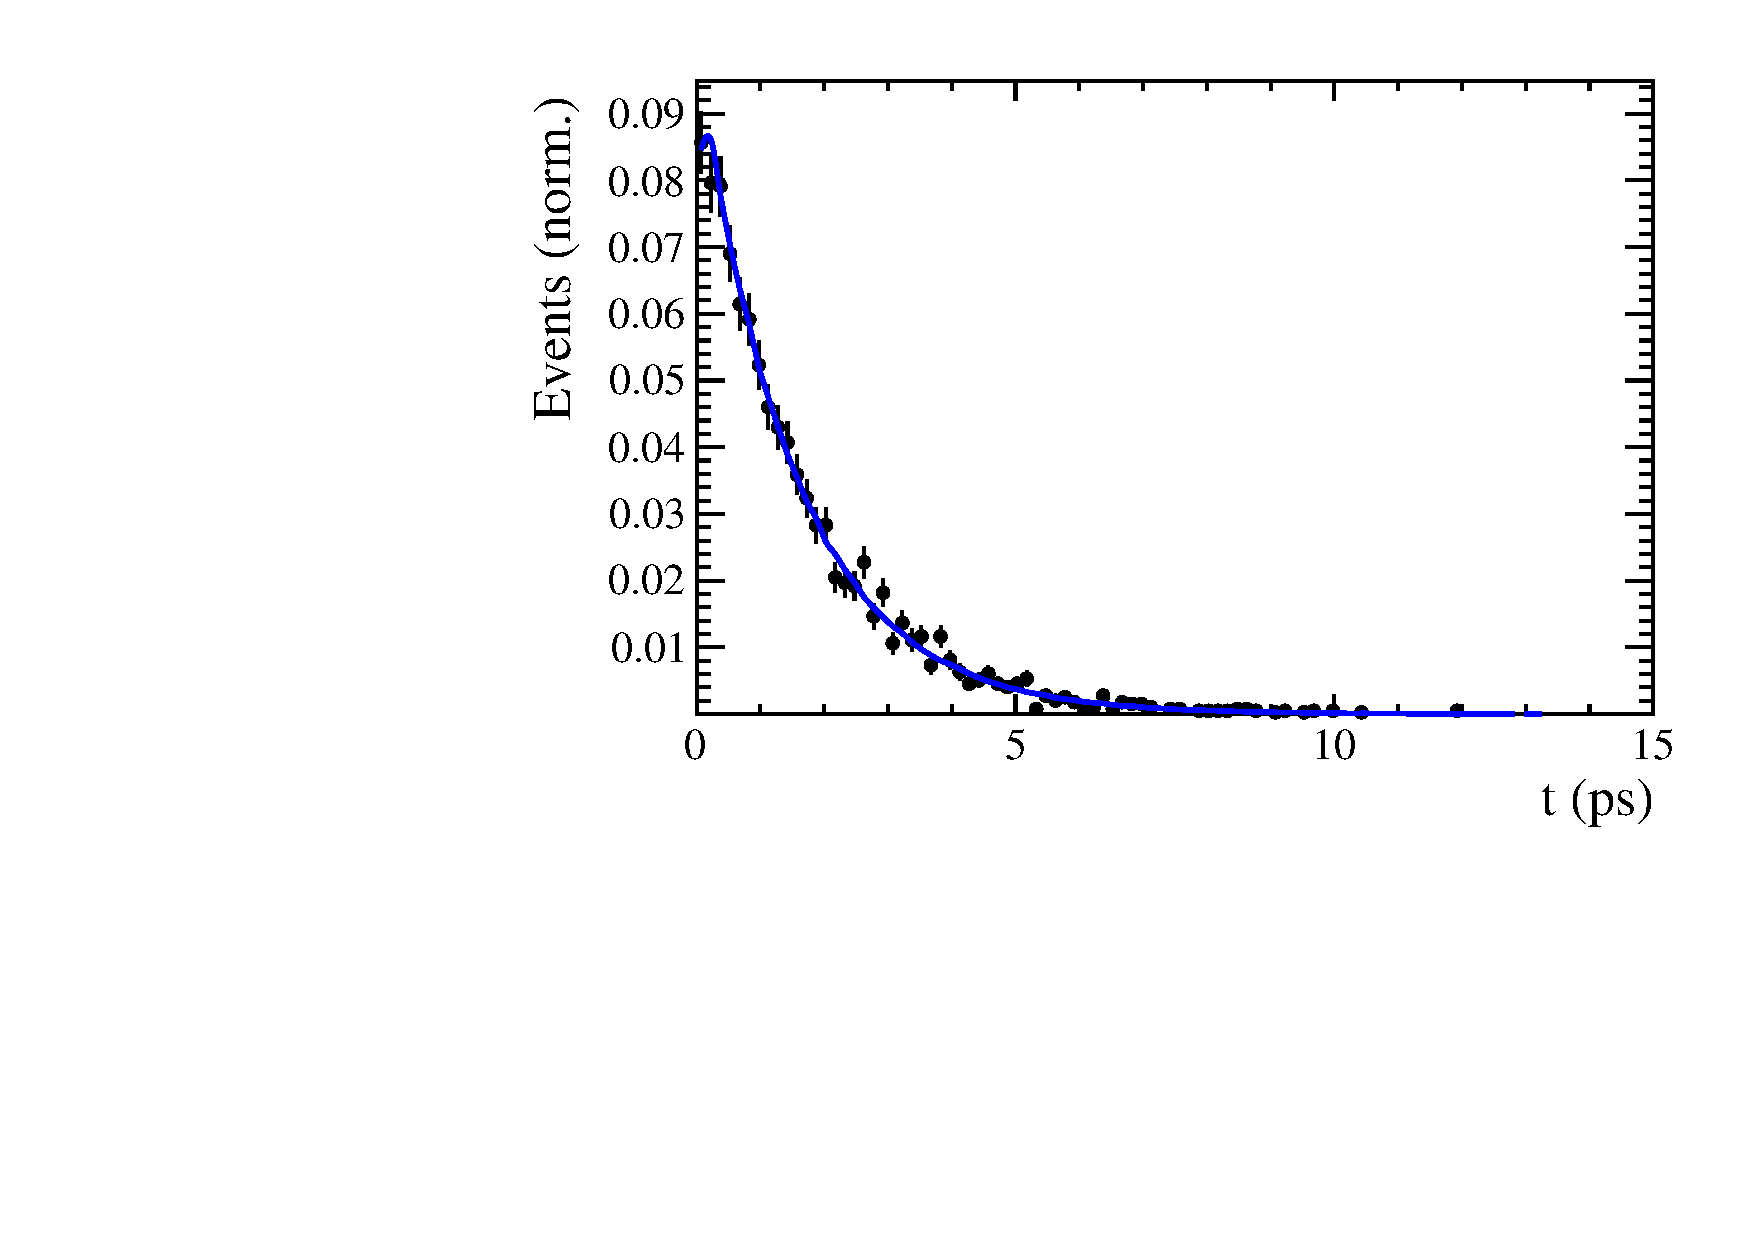
\includegraphics[width=0.45\textwidth, height = !]{figs/timeFit/signal_DsKpipi_CPV_MC/h_t.pdf} 
		%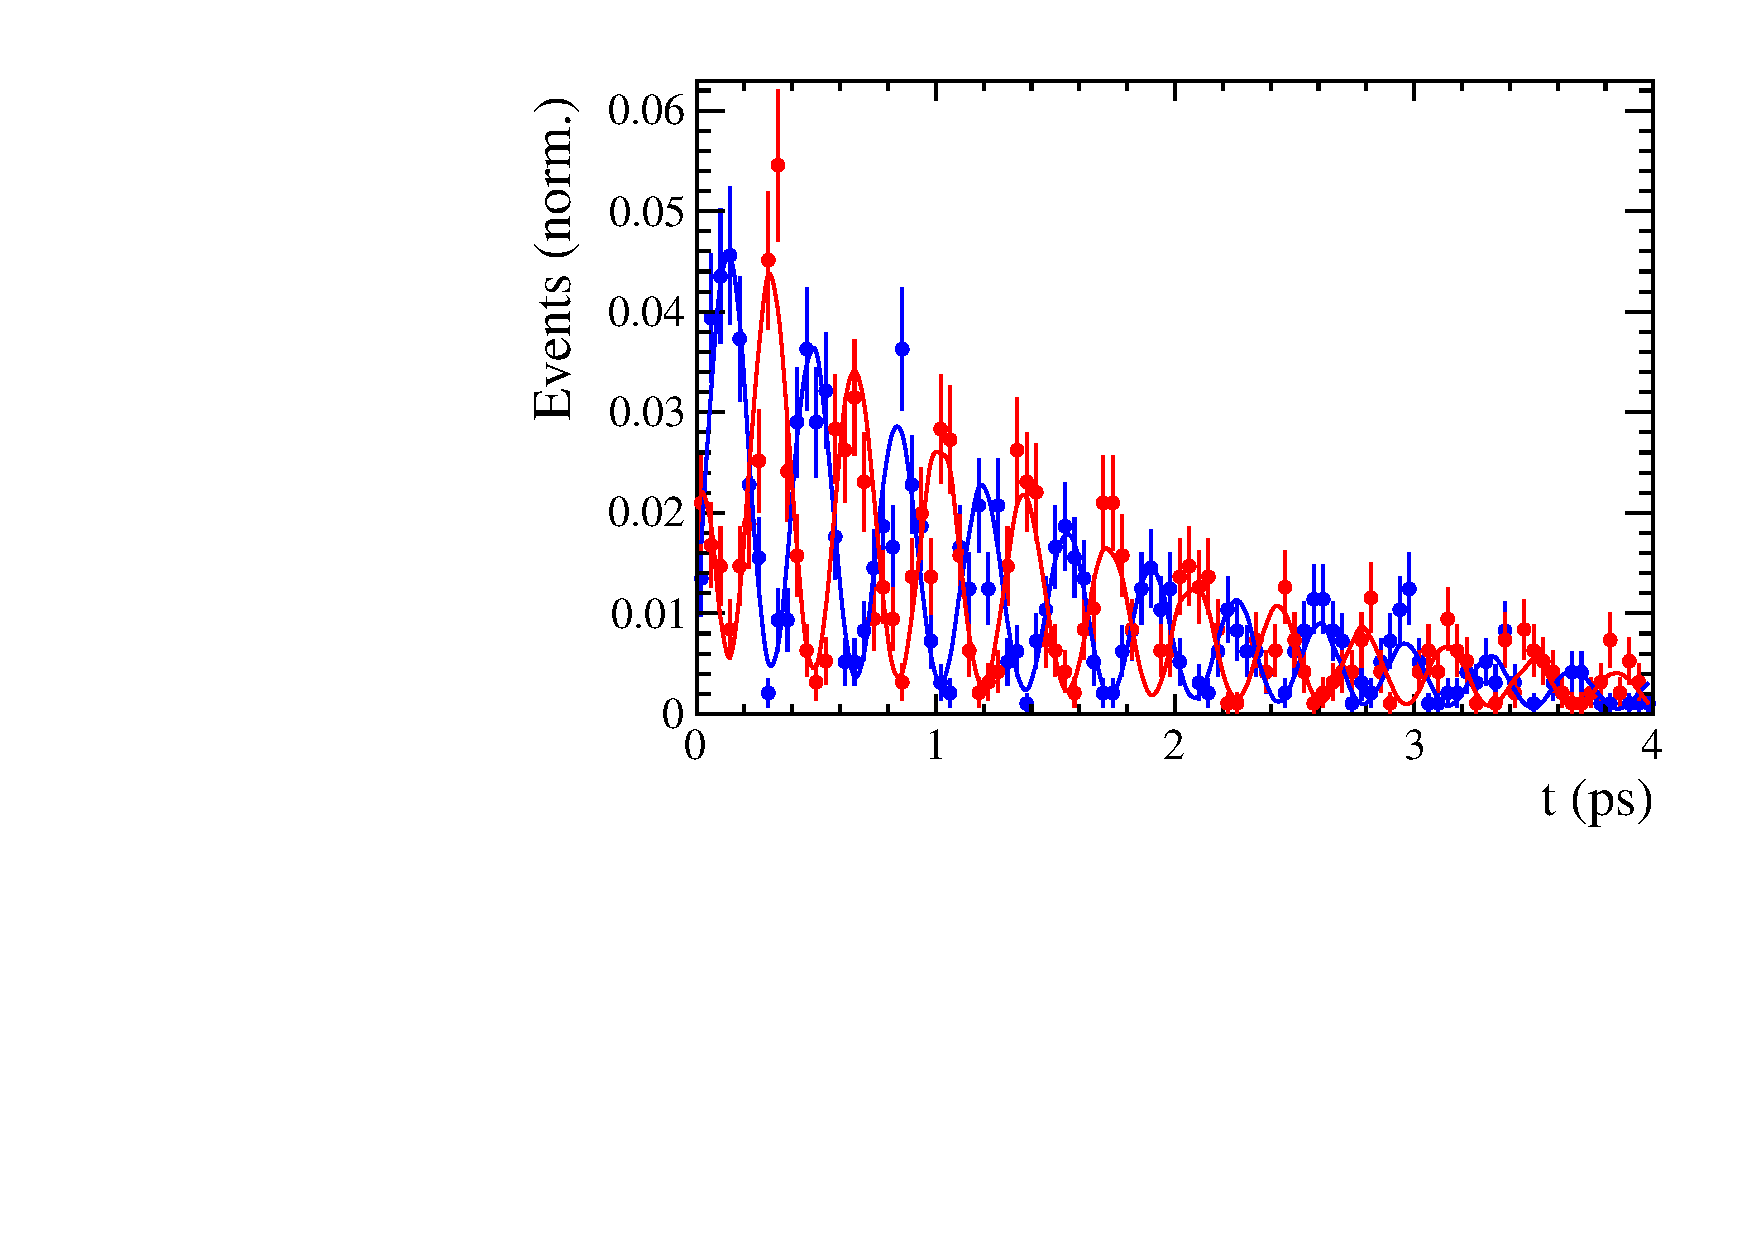
\includegraphics[width=0.32\textwidth, height = !]{figs/timeFit/signal_DsKpipi_CPV_MC/h_t_mixed_m.pdf} 	
		%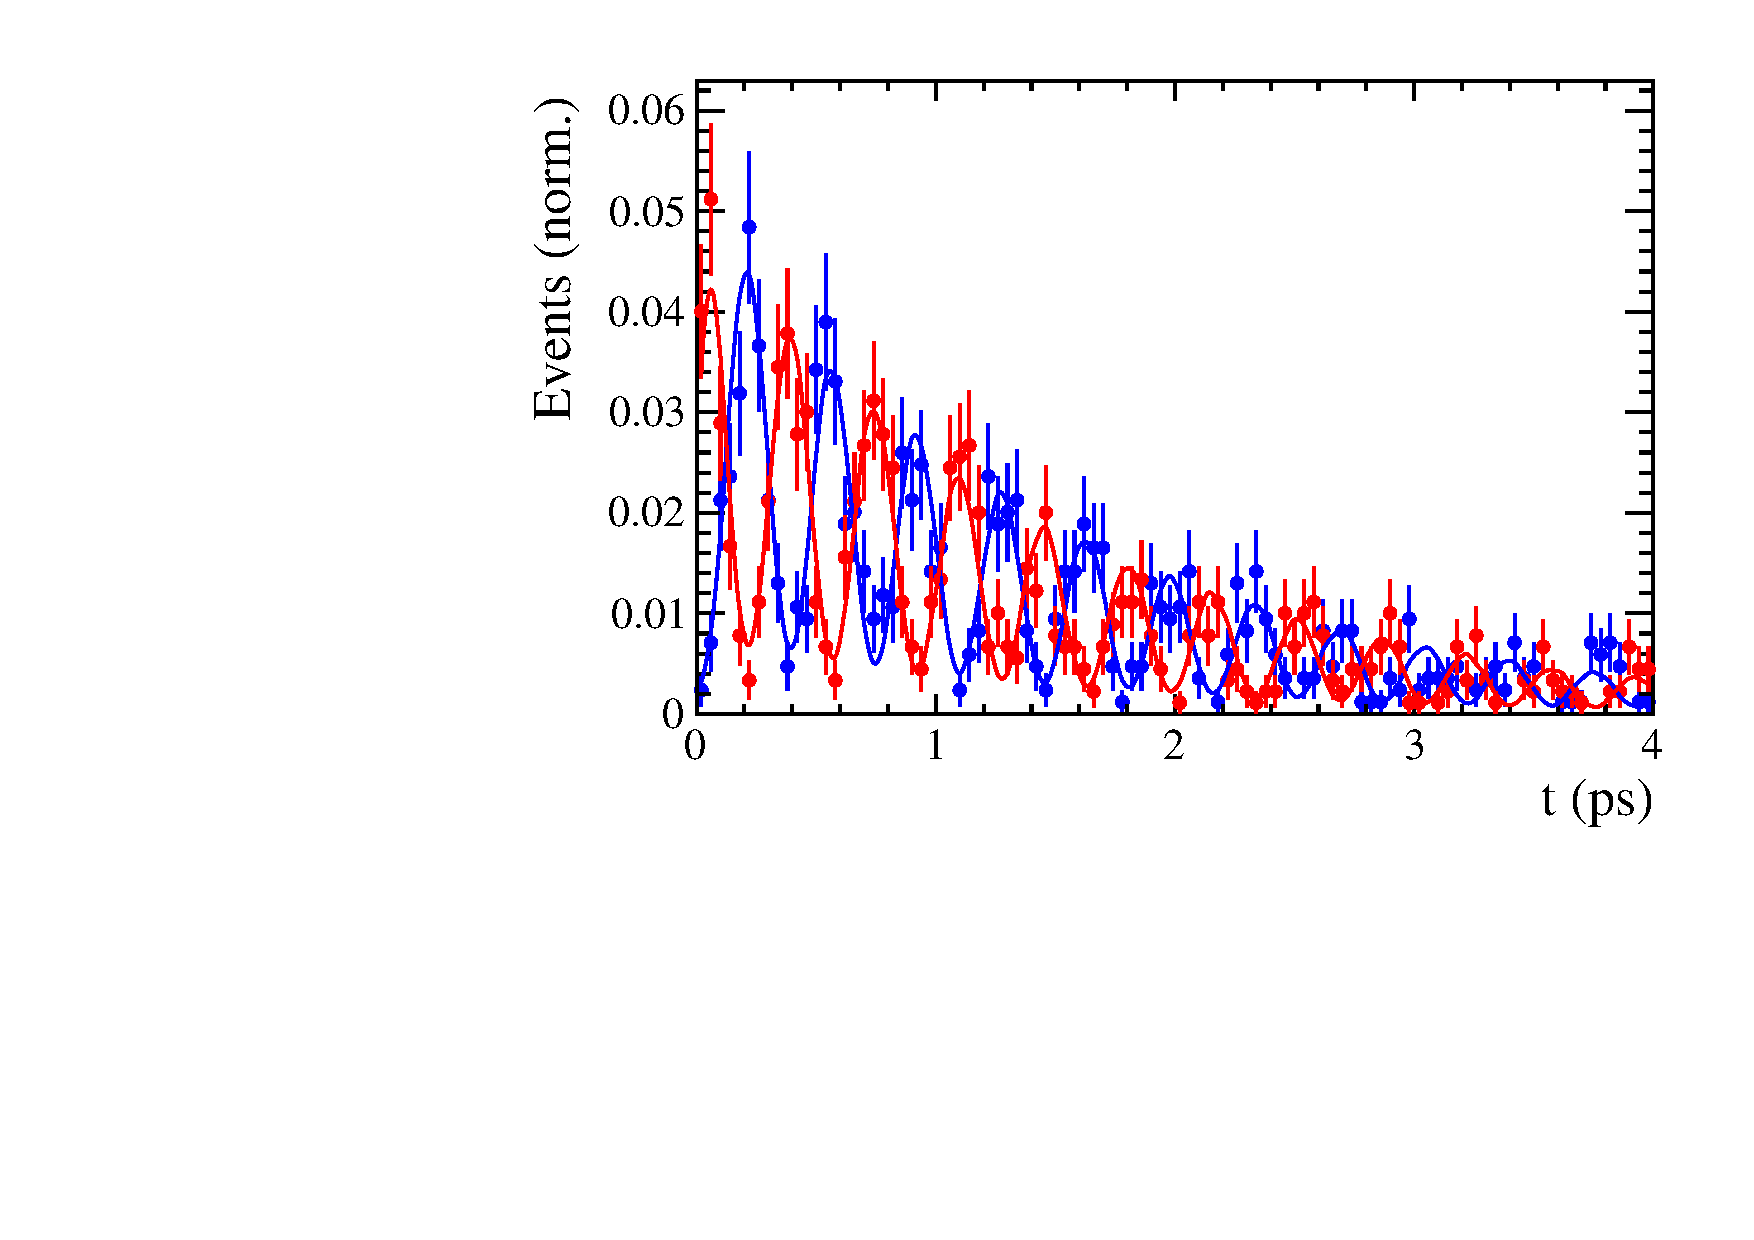
\includegraphics[width=0.32\textwidth, height = !]{figs/timeFit/signal_DsKpipi_CPV_MC/h_t_mixed_p.pdf} 
		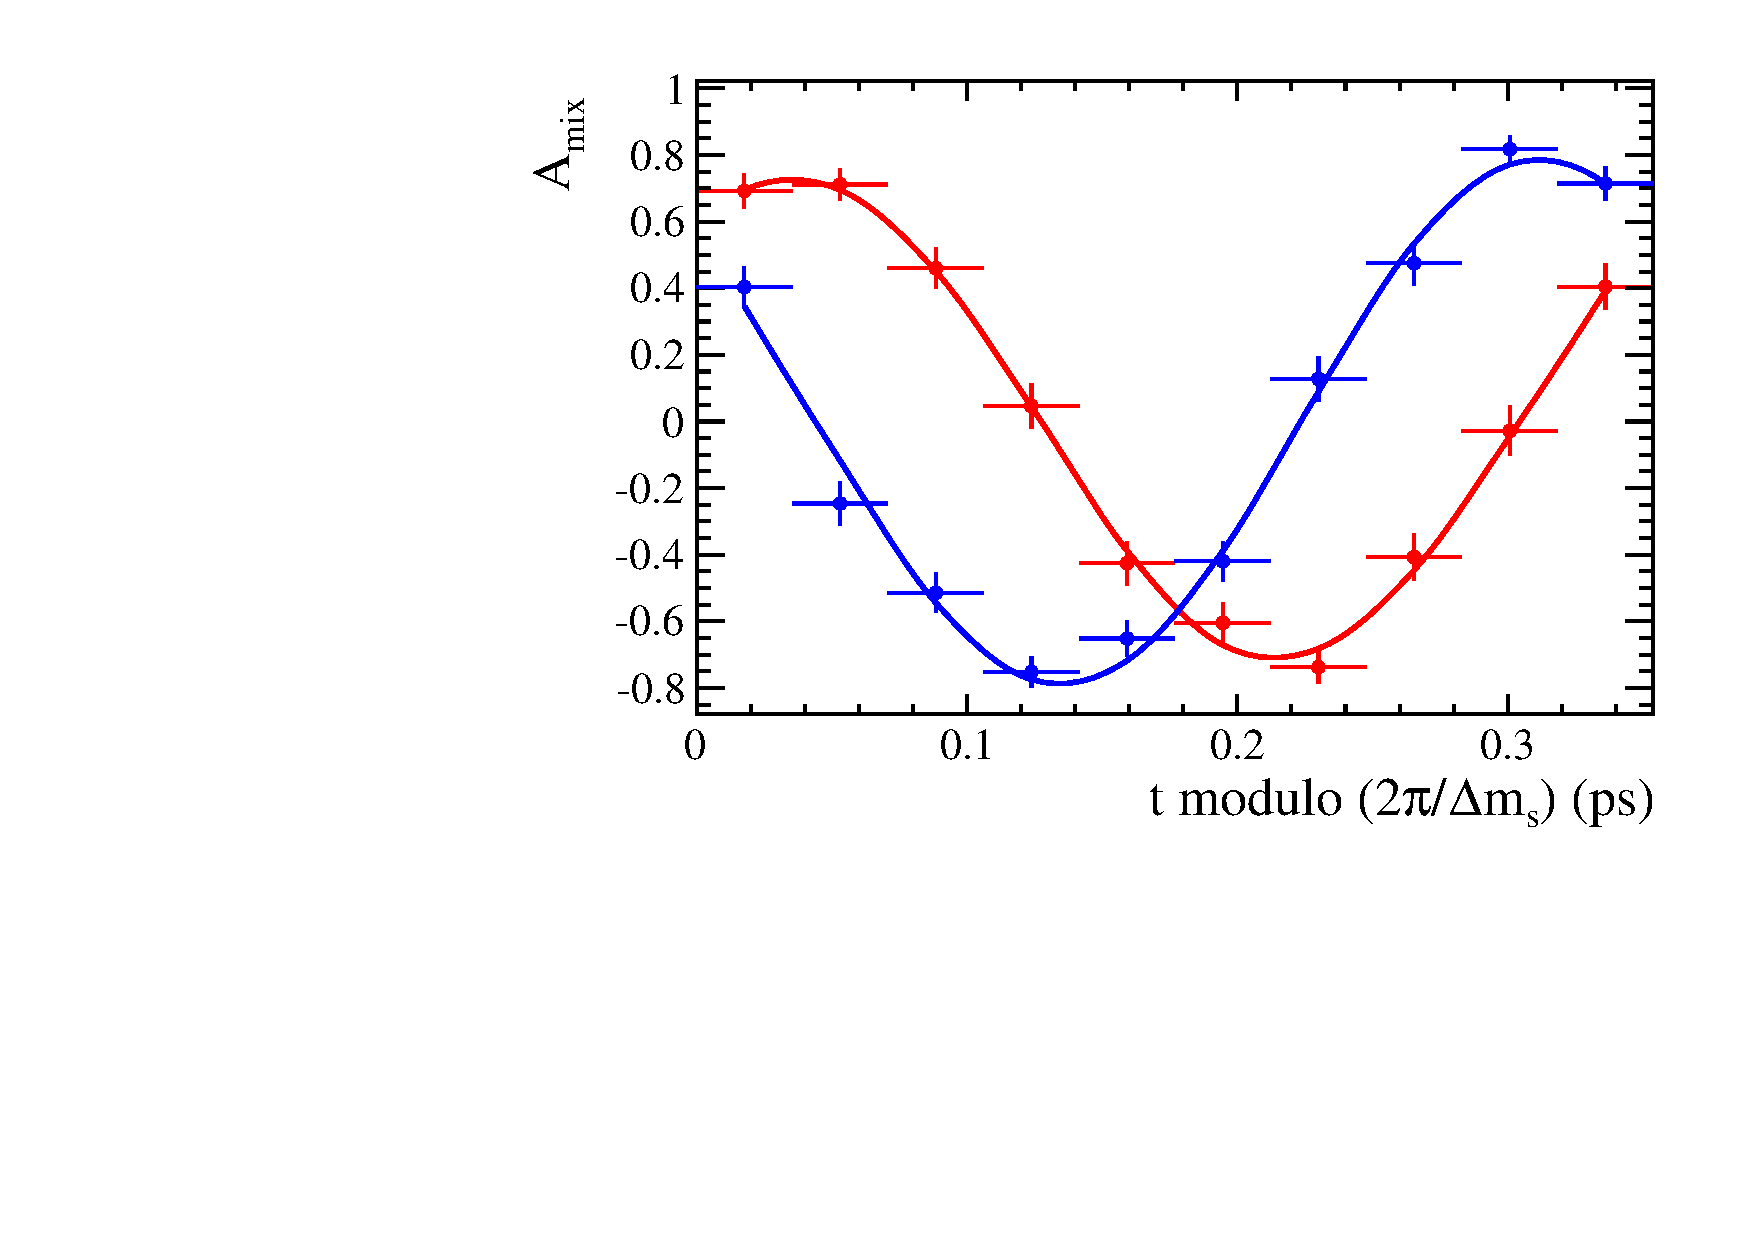
\includegraphics[width=0.45\textwidth, height = !]{figs/timeFit/signal_DsKpipi_CPV_MC/h_asym.pdf} 
		
		\caption{Left: Time distribution of $B_s \to D_s K \pi\pi$ events generated with \textsf{EVTGEN} (points with error bars) and \textsf{MINT2} fit projections (solid line). 
                  Right: Time-dependent asymmetry between mixed and unmixed events folded into one oscillation period for 
                  $D_s^- K^+ \pi\pi$ (red) and $D_s^+ K^- \pi\pi$ (blue) final states.
                  The data points show events generated with \textsf{EVTGEN}, while the solid lines show the \textsf{MINT2} fit projections.}
		\label{fig:FitGenMC}	
\end{figure}	

\begin{figure}[h]
	\centering
		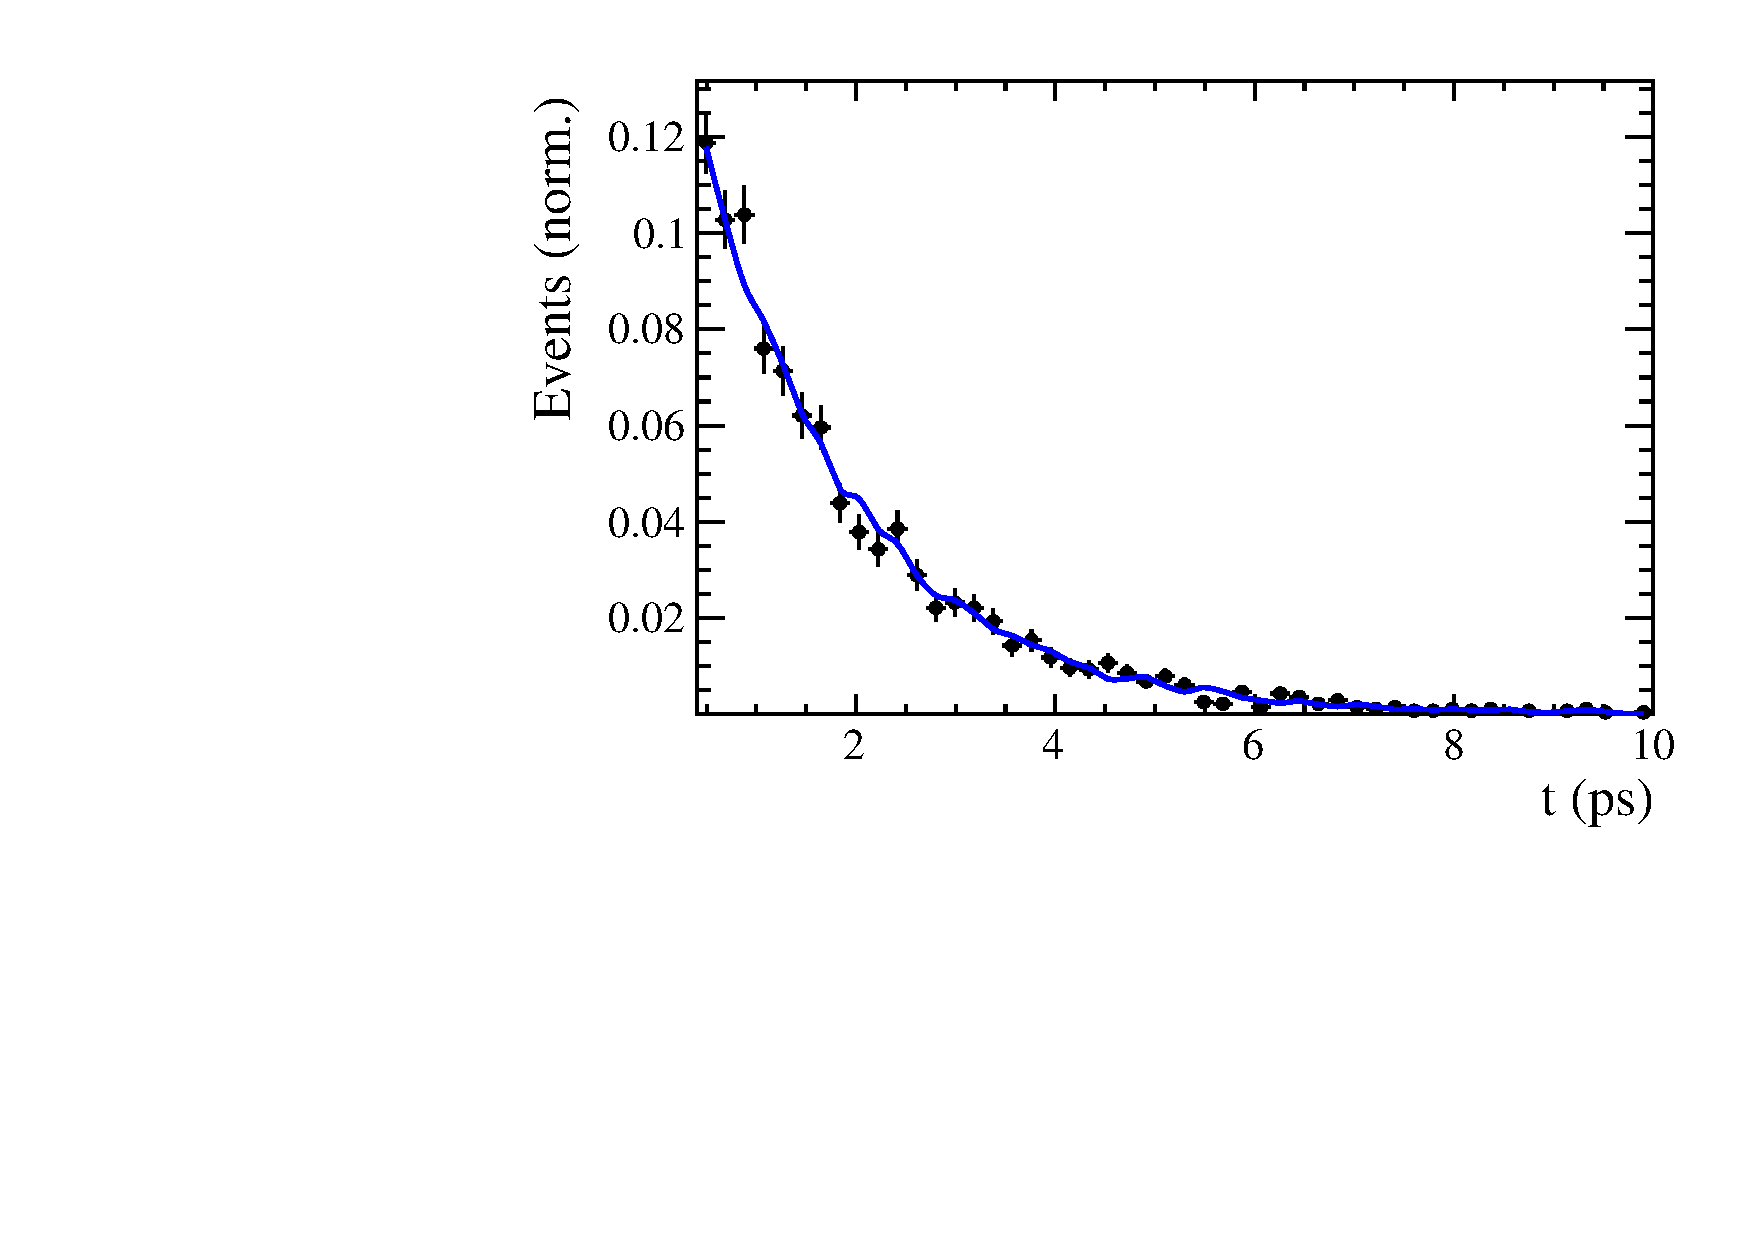
\includegraphics[width=0.32\textwidth, height = !]{figs/fullFit/signal_DsKpipi_CPV_MC/h_t.pdf} 
		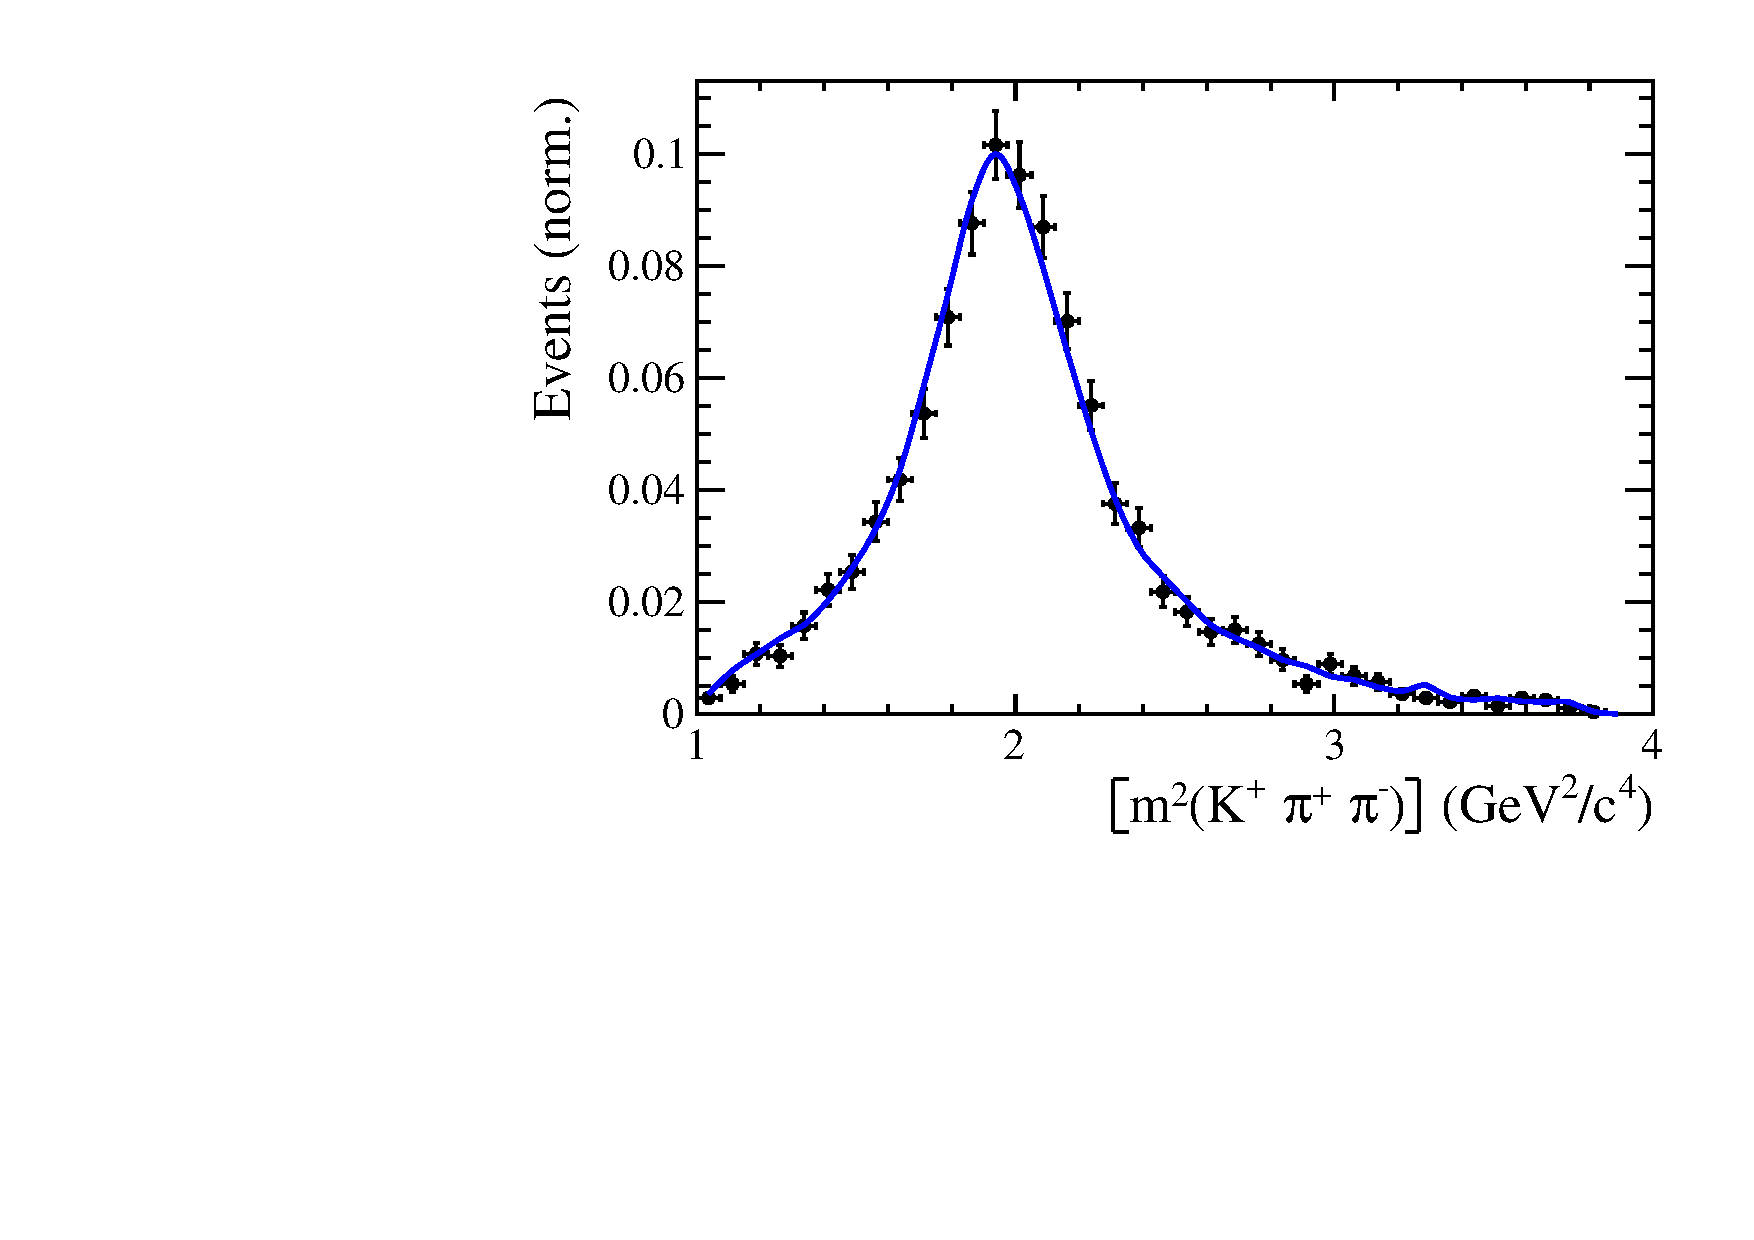
\includegraphics[width=0.32\textwidth, height = !]{figs/fullFit/signal_DsKpipi_CPV_MC/s_Kpipi.pdf} 
		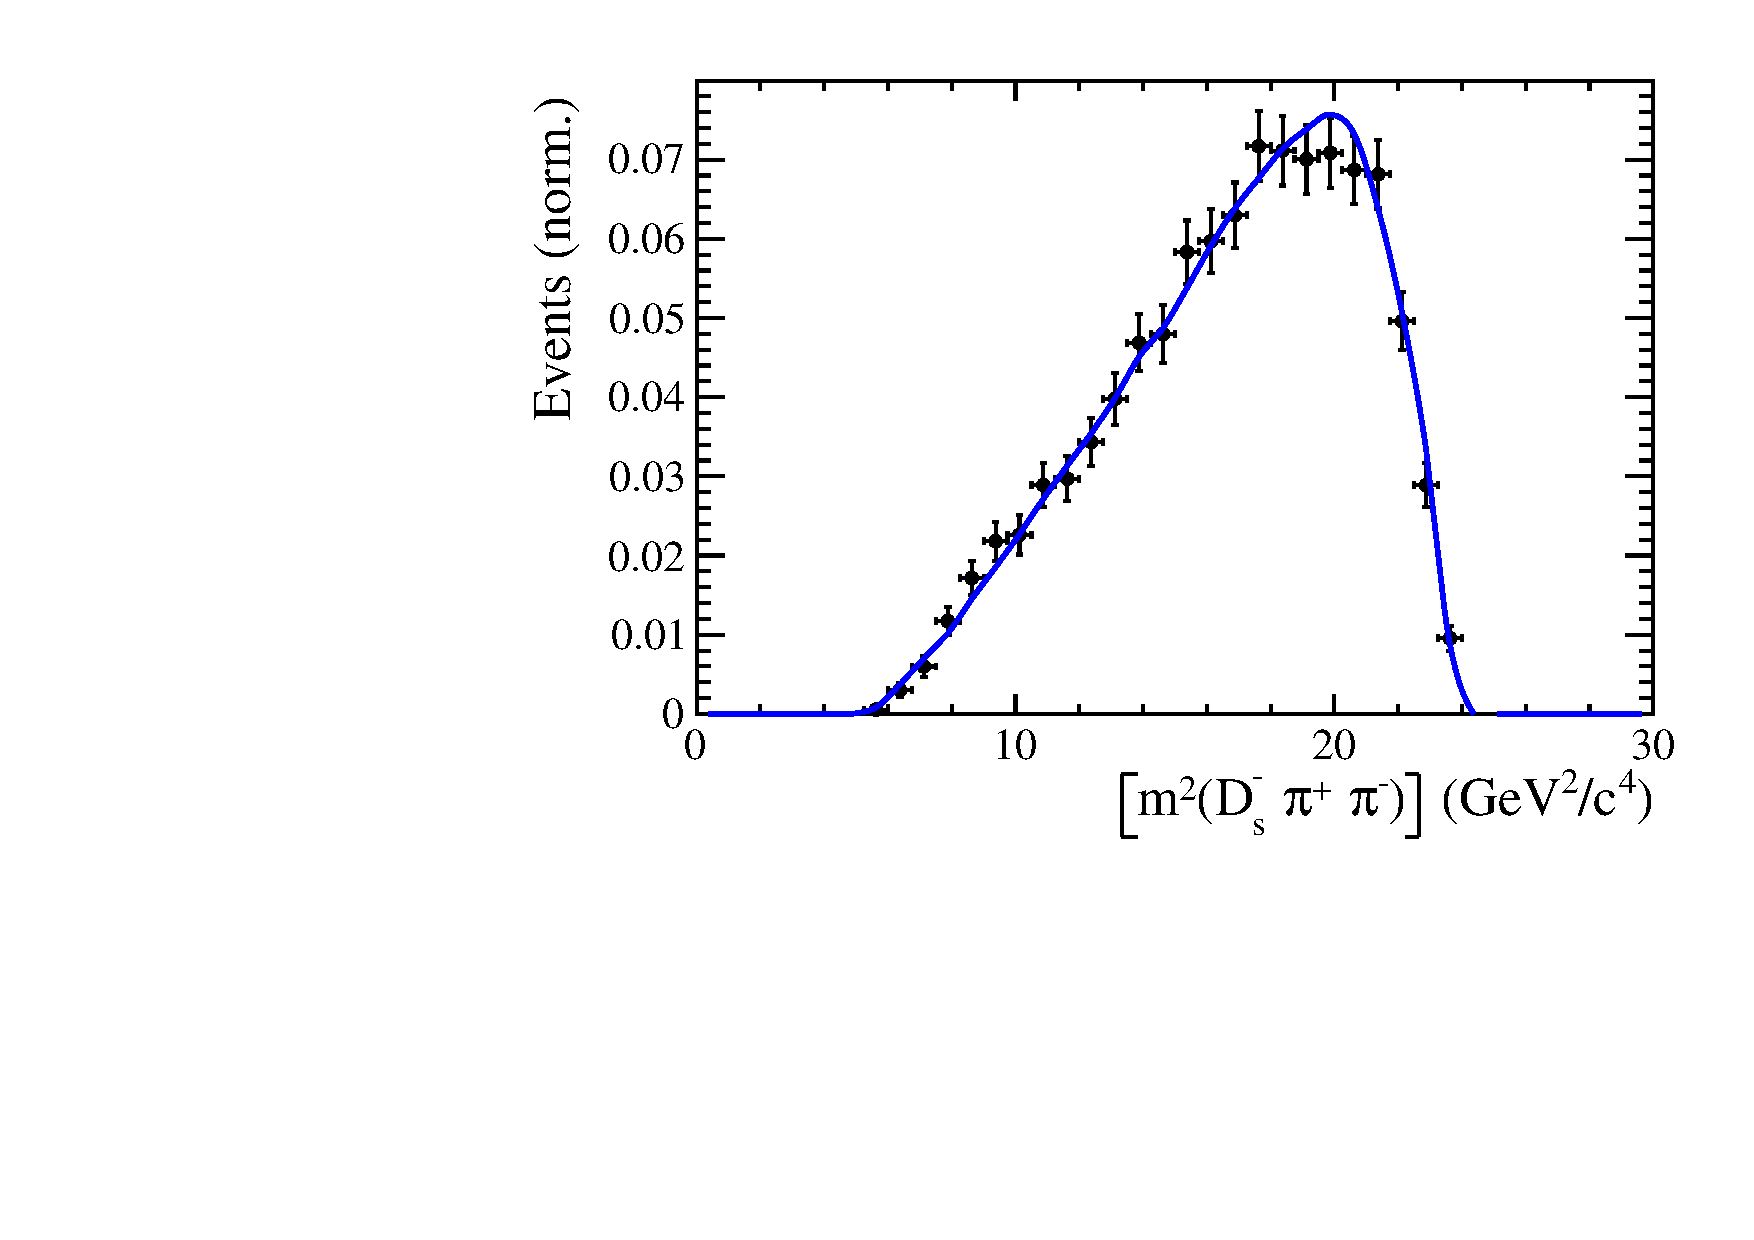
\includegraphics[width=0.32\textwidth, height = !]{figs/fullFit/signal_DsKpipi_CPV_MC/s_Dspipi.pdf} 

		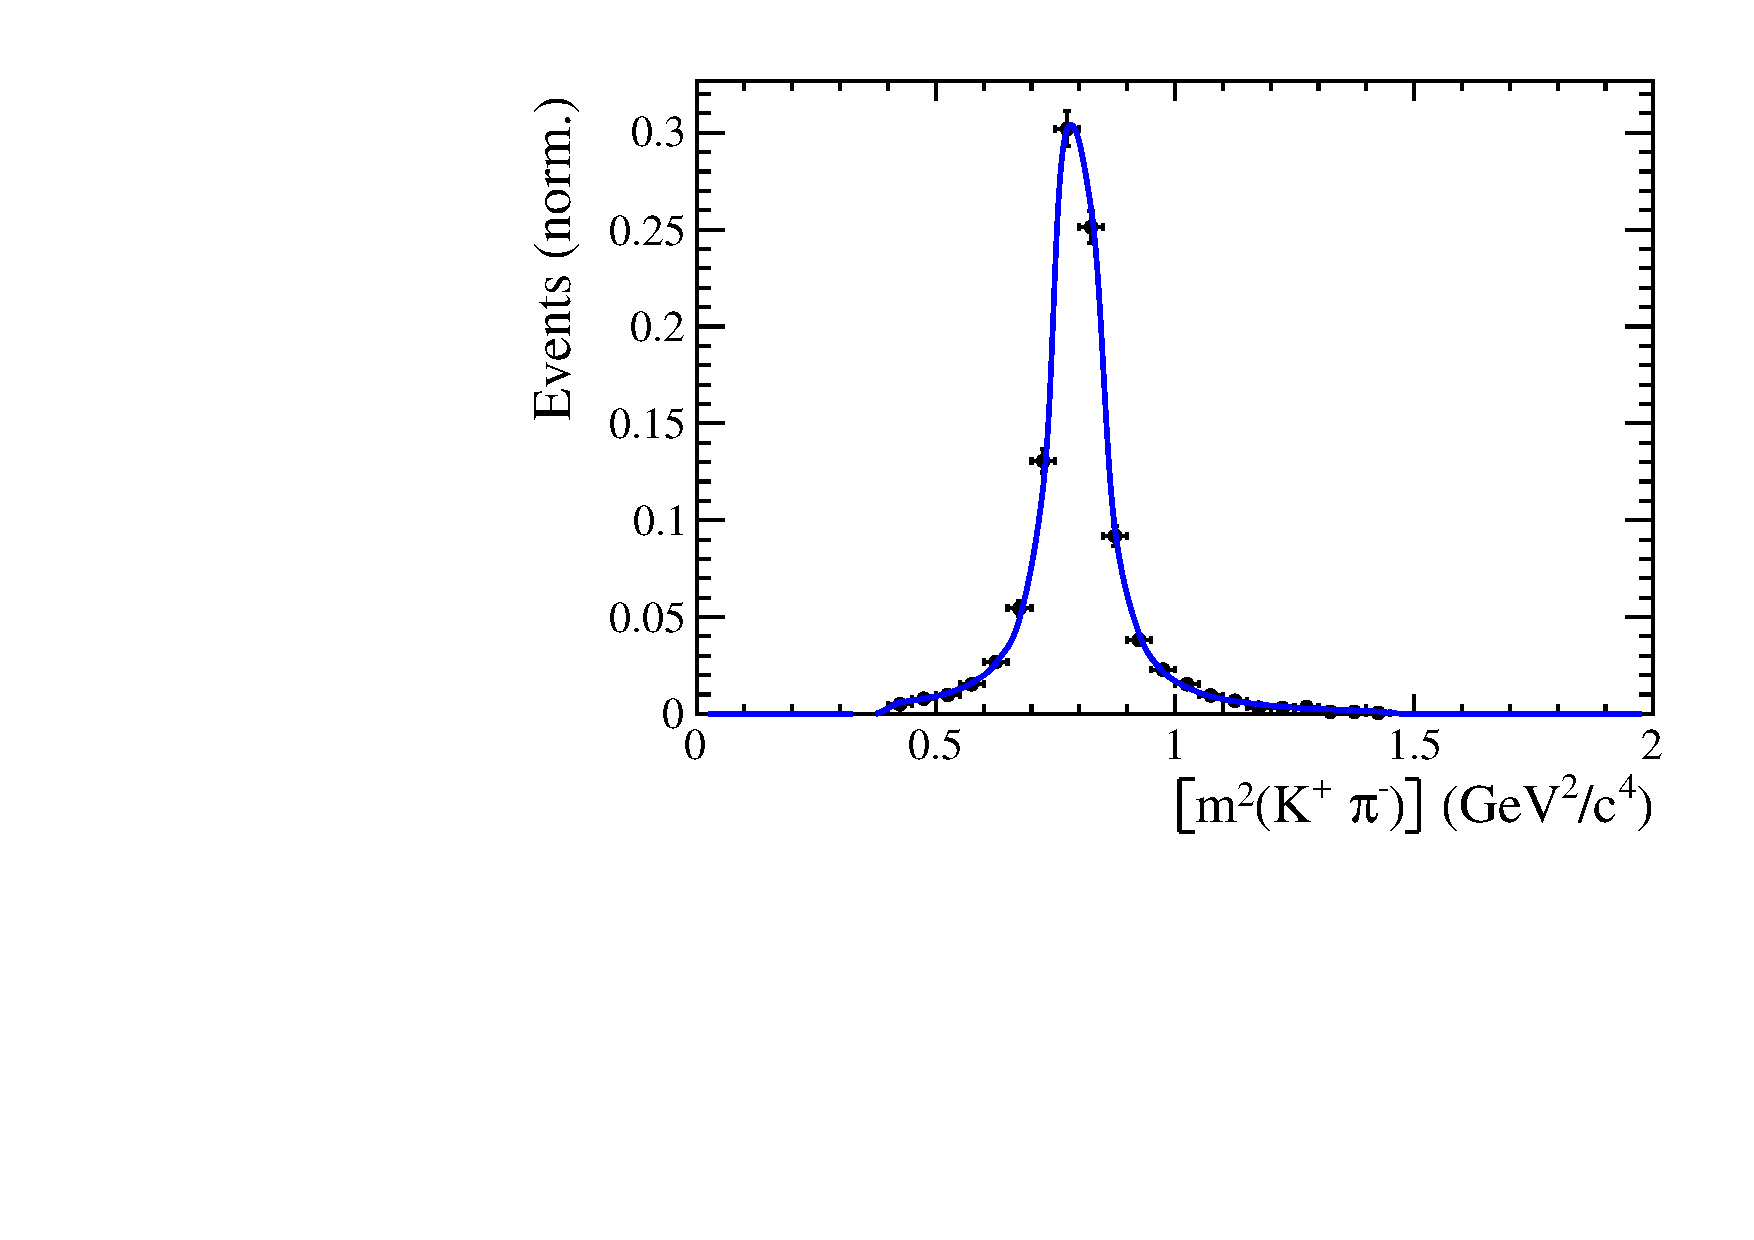
\includegraphics[width=0.32\textwidth, height = !]{figs/fullFit/signal_DsKpipi_CPV_MC/s_Kpi.pdf} 
		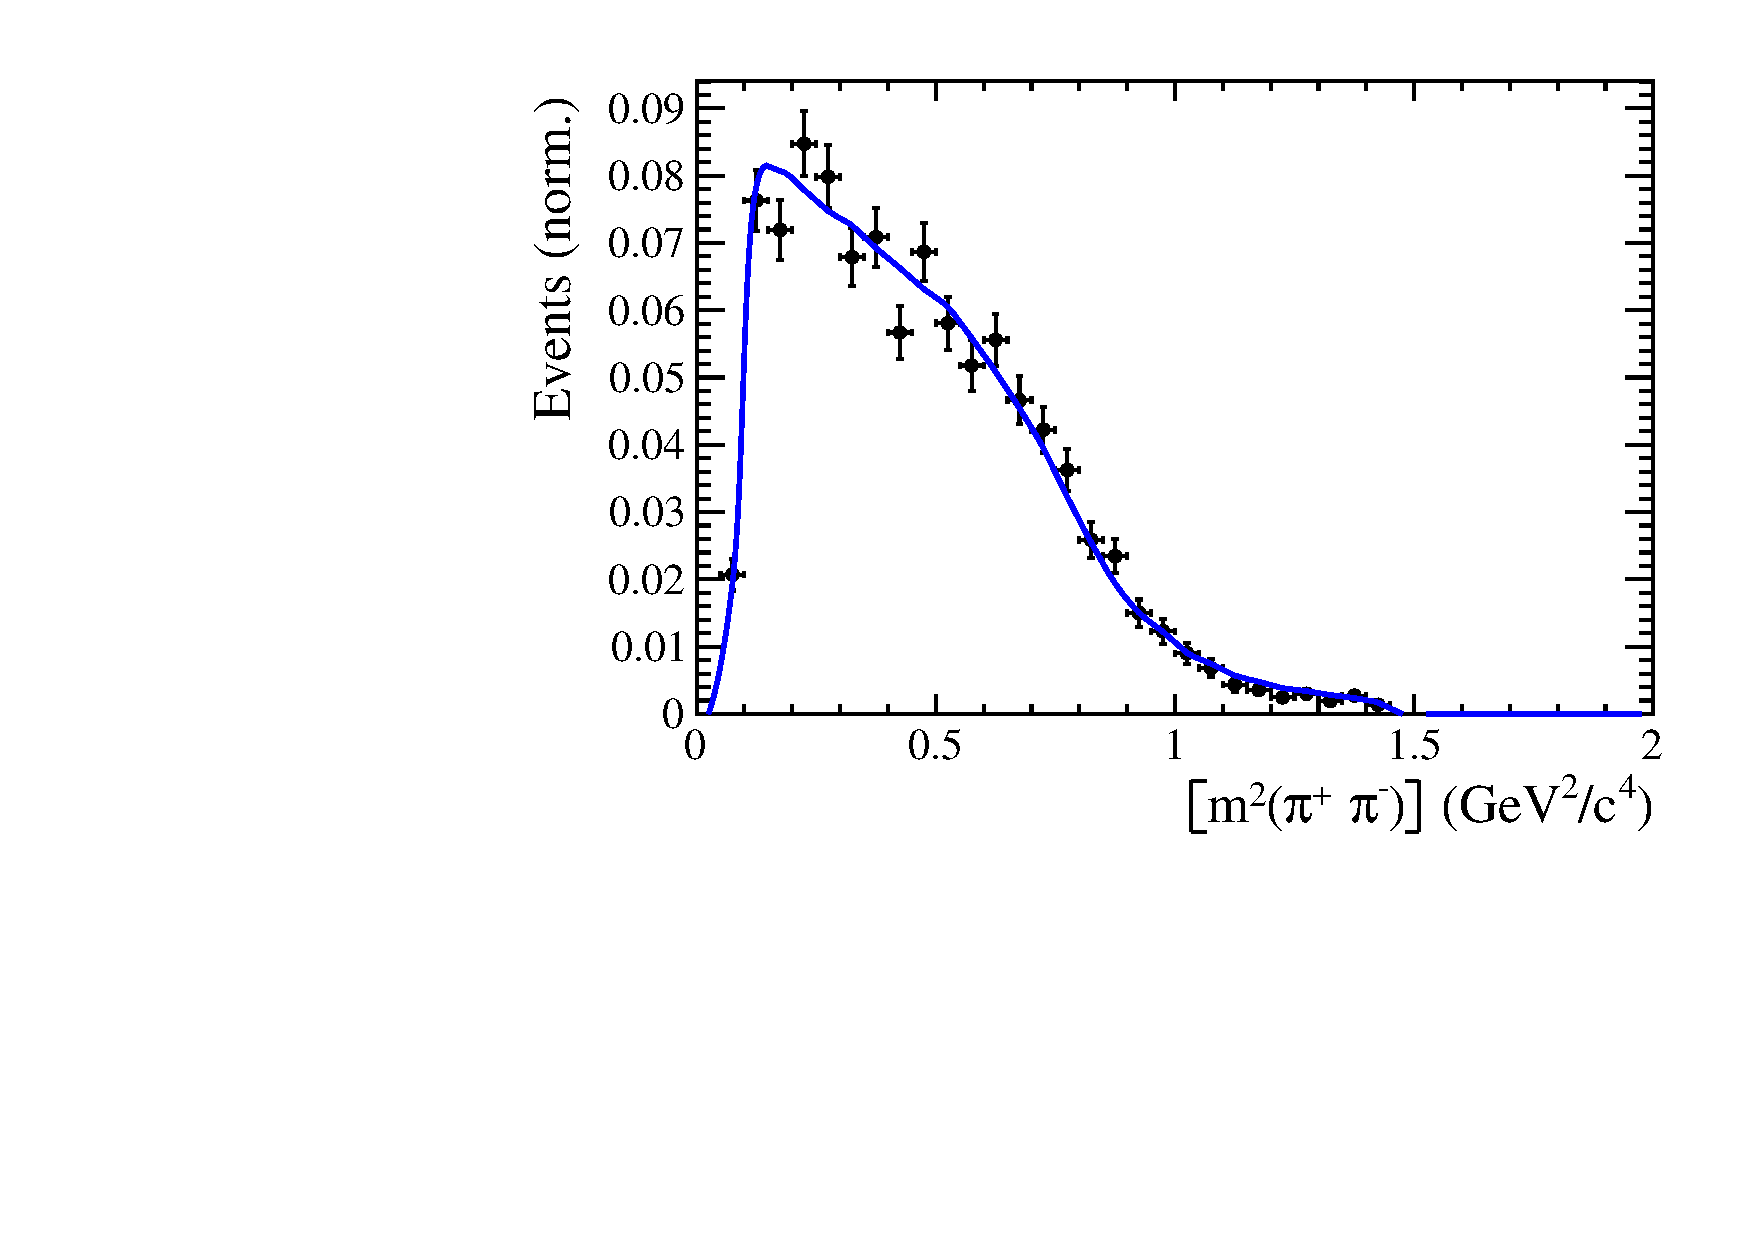
\includegraphics[width=0.32\textwidth, height = !]{figs/fullFit/signal_DsKpipi_CPV_MC/s_pipi.pdf} 
		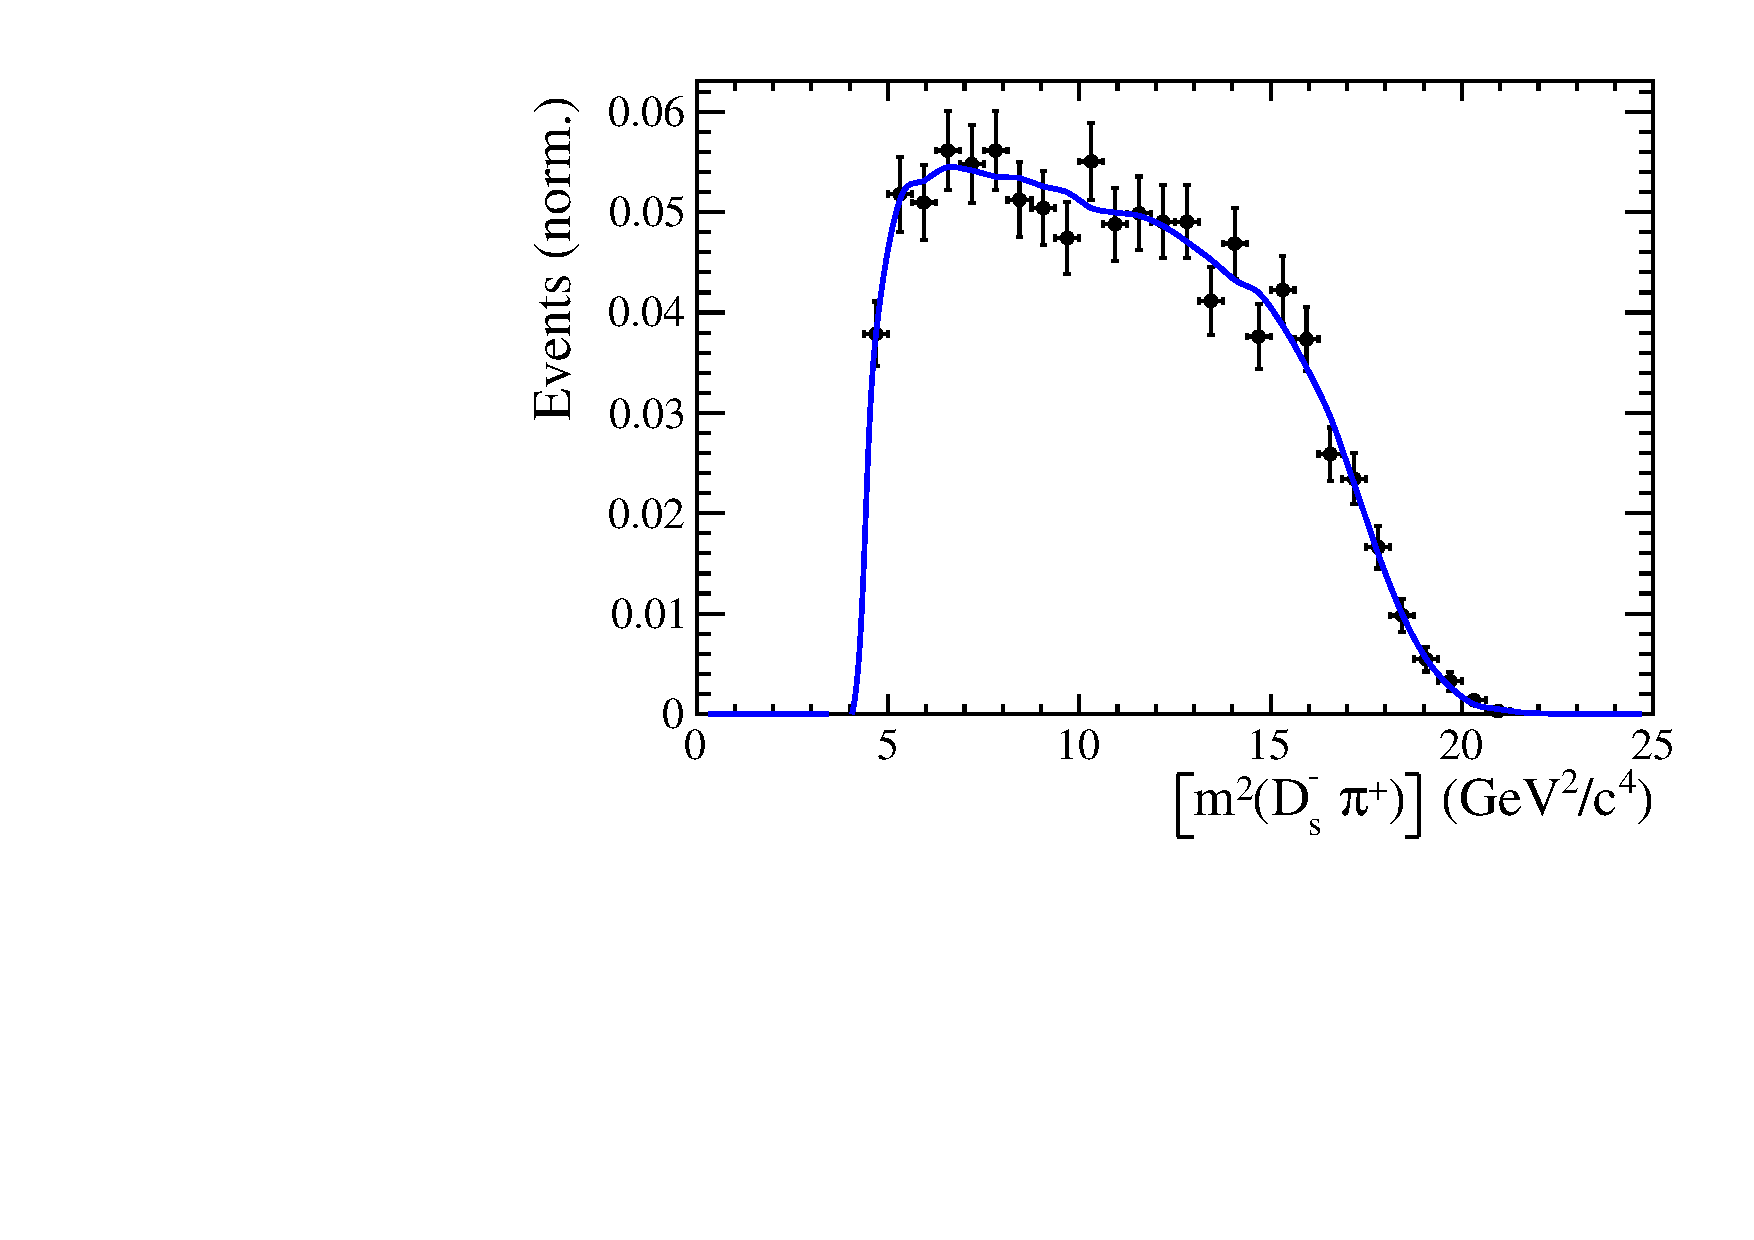
\includegraphics[width=0.32\textwidth, height = !]{figs/fullFit/signal_DsKpipi_CPV_MC/s_Dspi.pdf} 
		
		\caption{Time and invariant mass distributions of $B_s \to D_s K \pi\pi$ events generated with \textsf{EVTGEN} (points with error bars) and \textsf{MINT2} fit projections (blue solid line).} 		
		\label{fig:FitGenMC2}	
\end{figure}	

\begin{figure}[h]
	\centering
		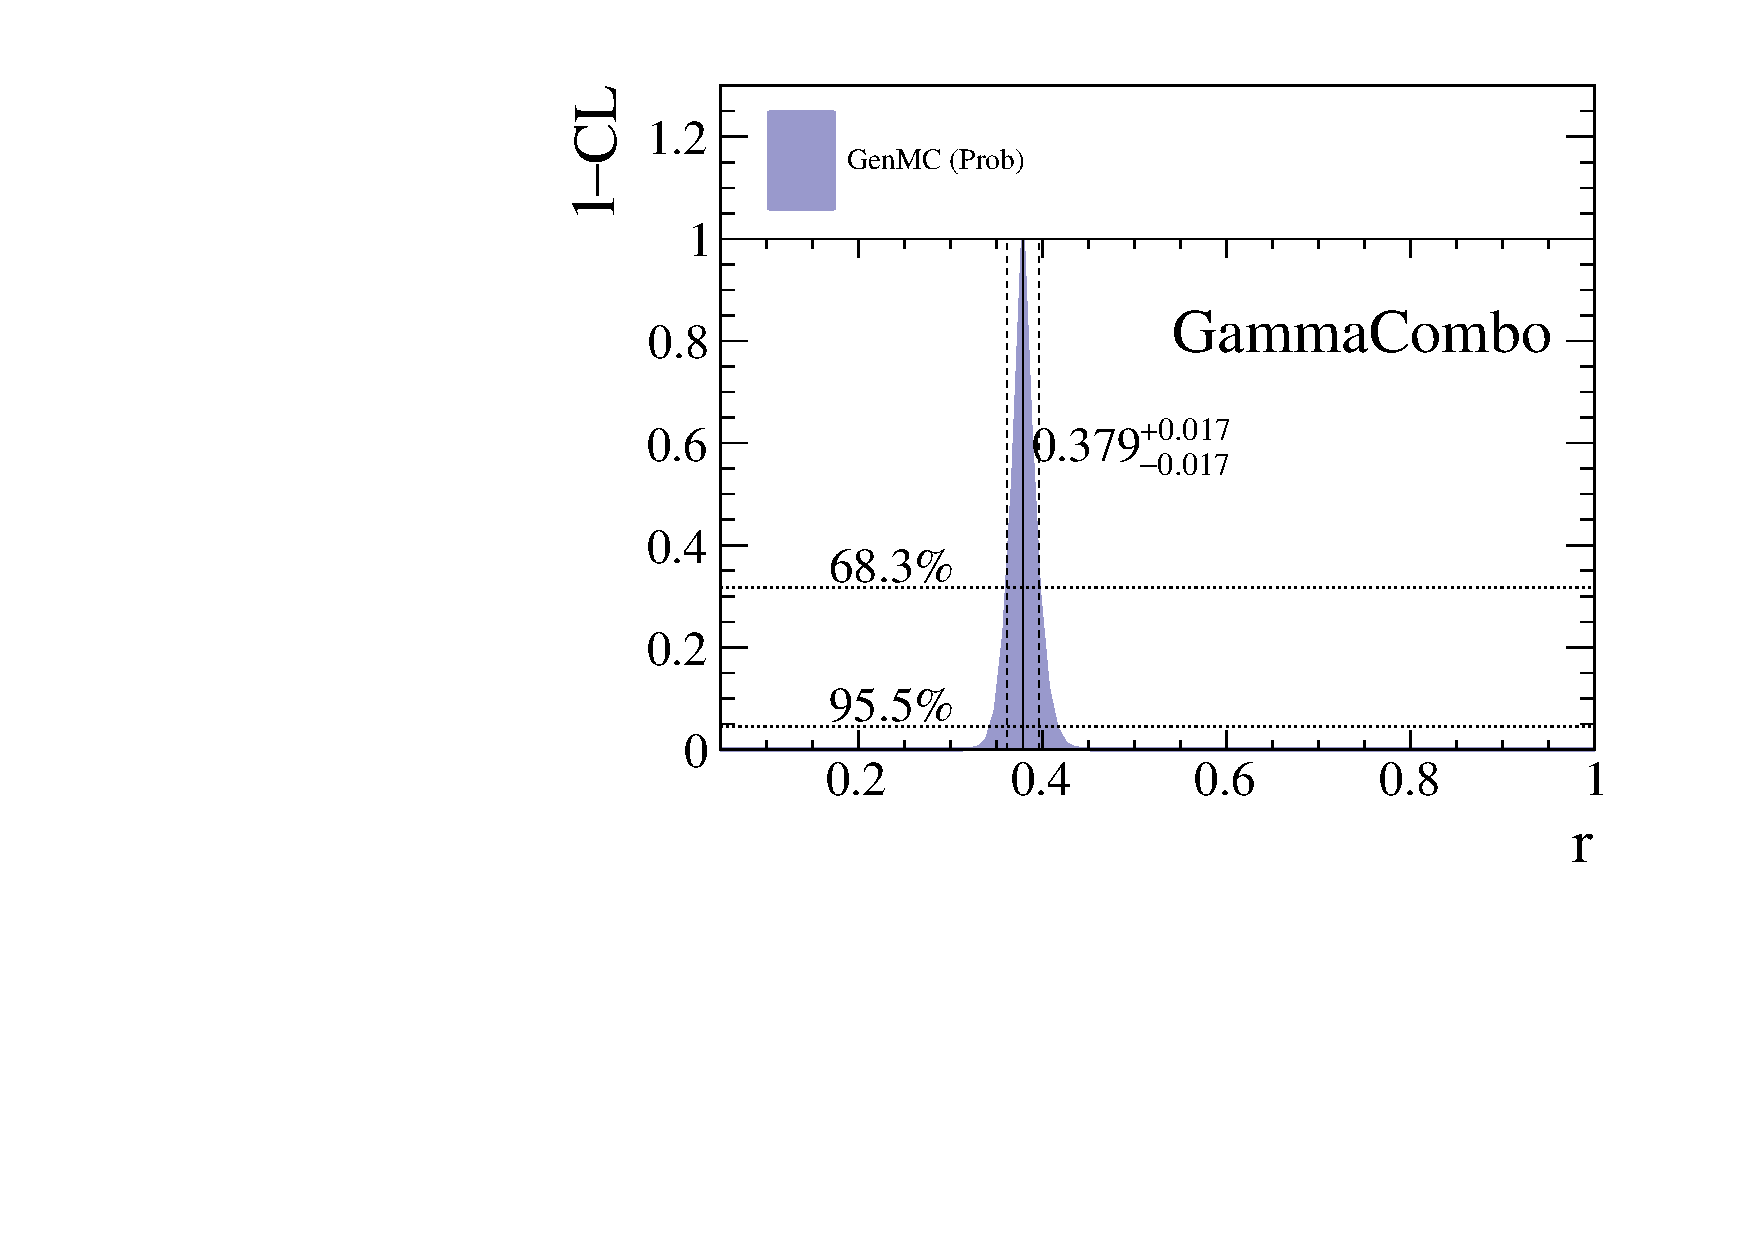
\includegraphics[width=0.4\textwidth, height = !]{figs/GammaCombo/signal_DsKpipi_CPV_MC/cartesian_cp_coeff_r.pdf} 
		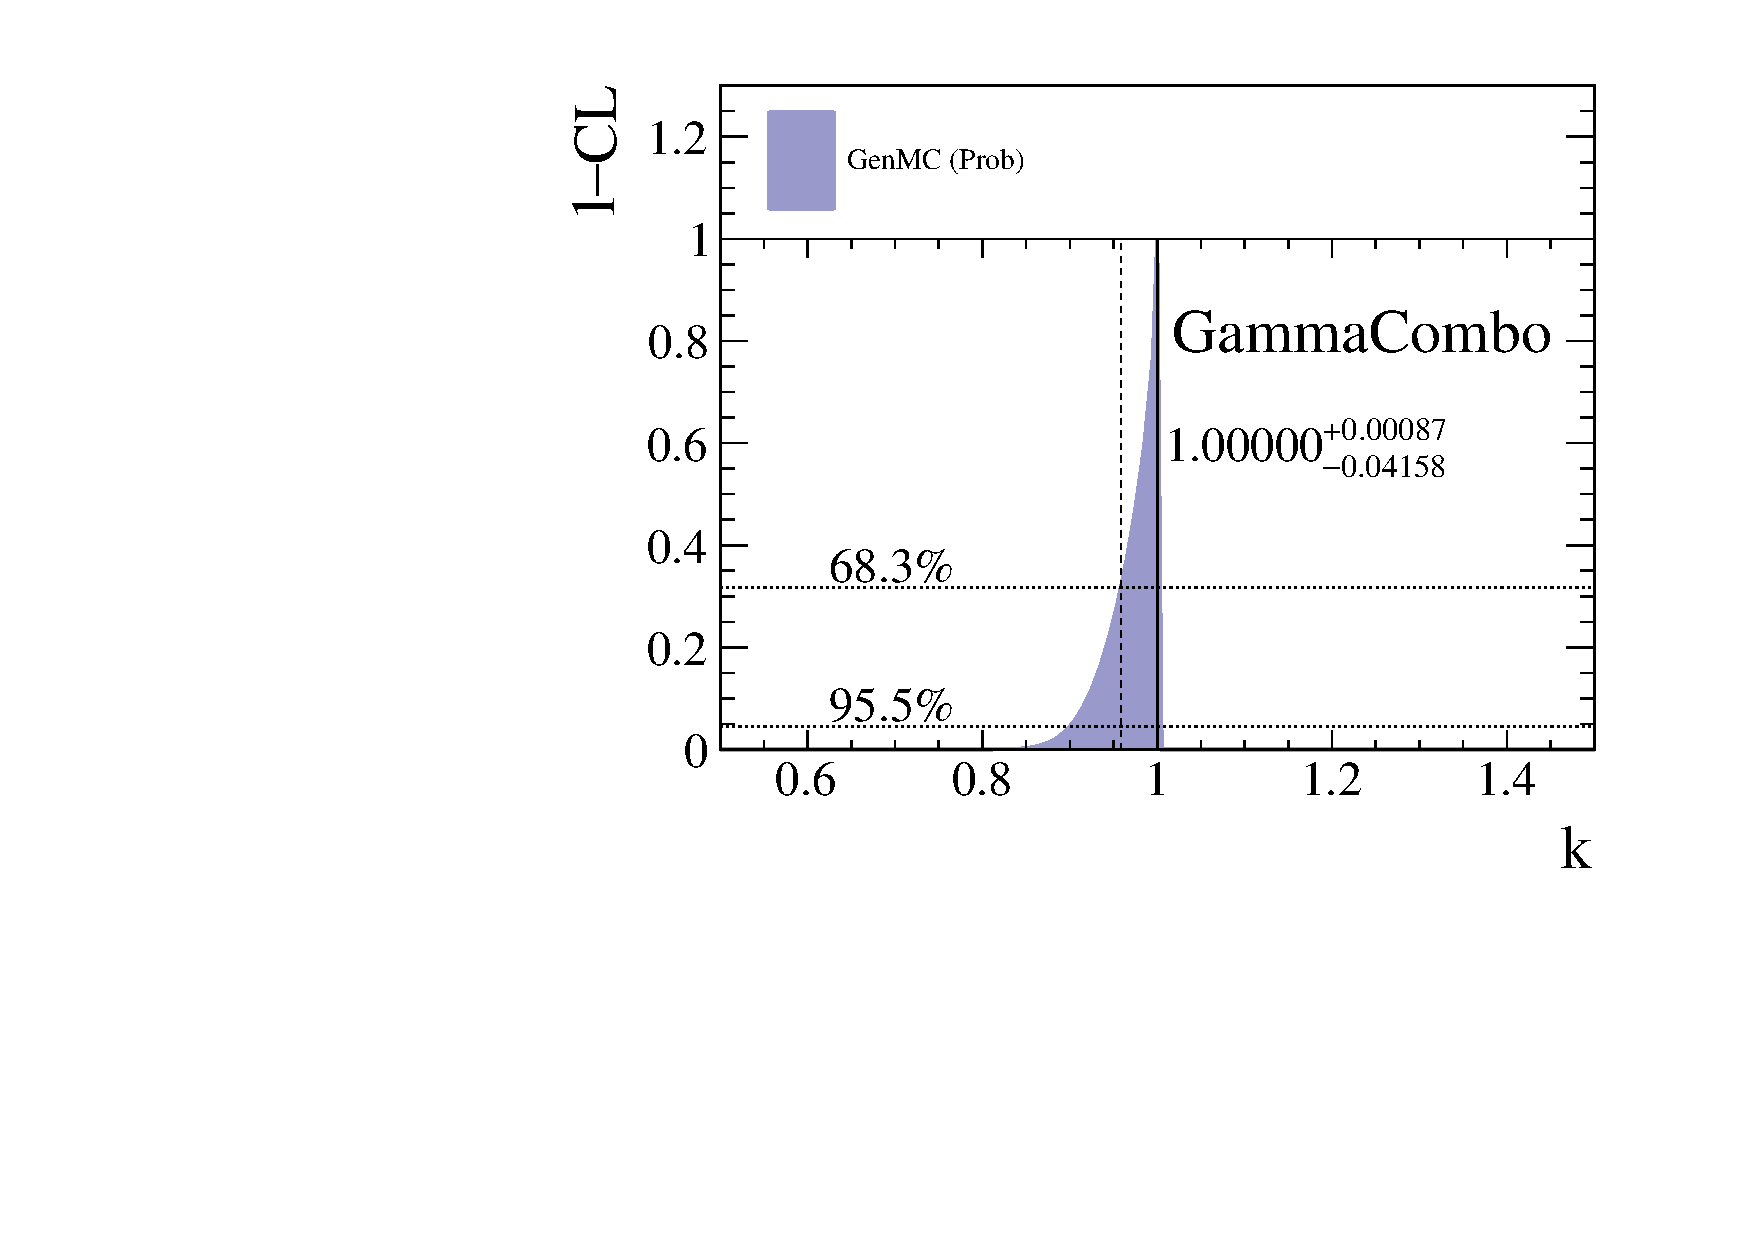
\includegraphics[width=0.4\textwidth, height = !]{figs/GammaCombo/signal_DsKpipi_CPV_MC/cartesian_cp_coeff_k.pdf} 
		
		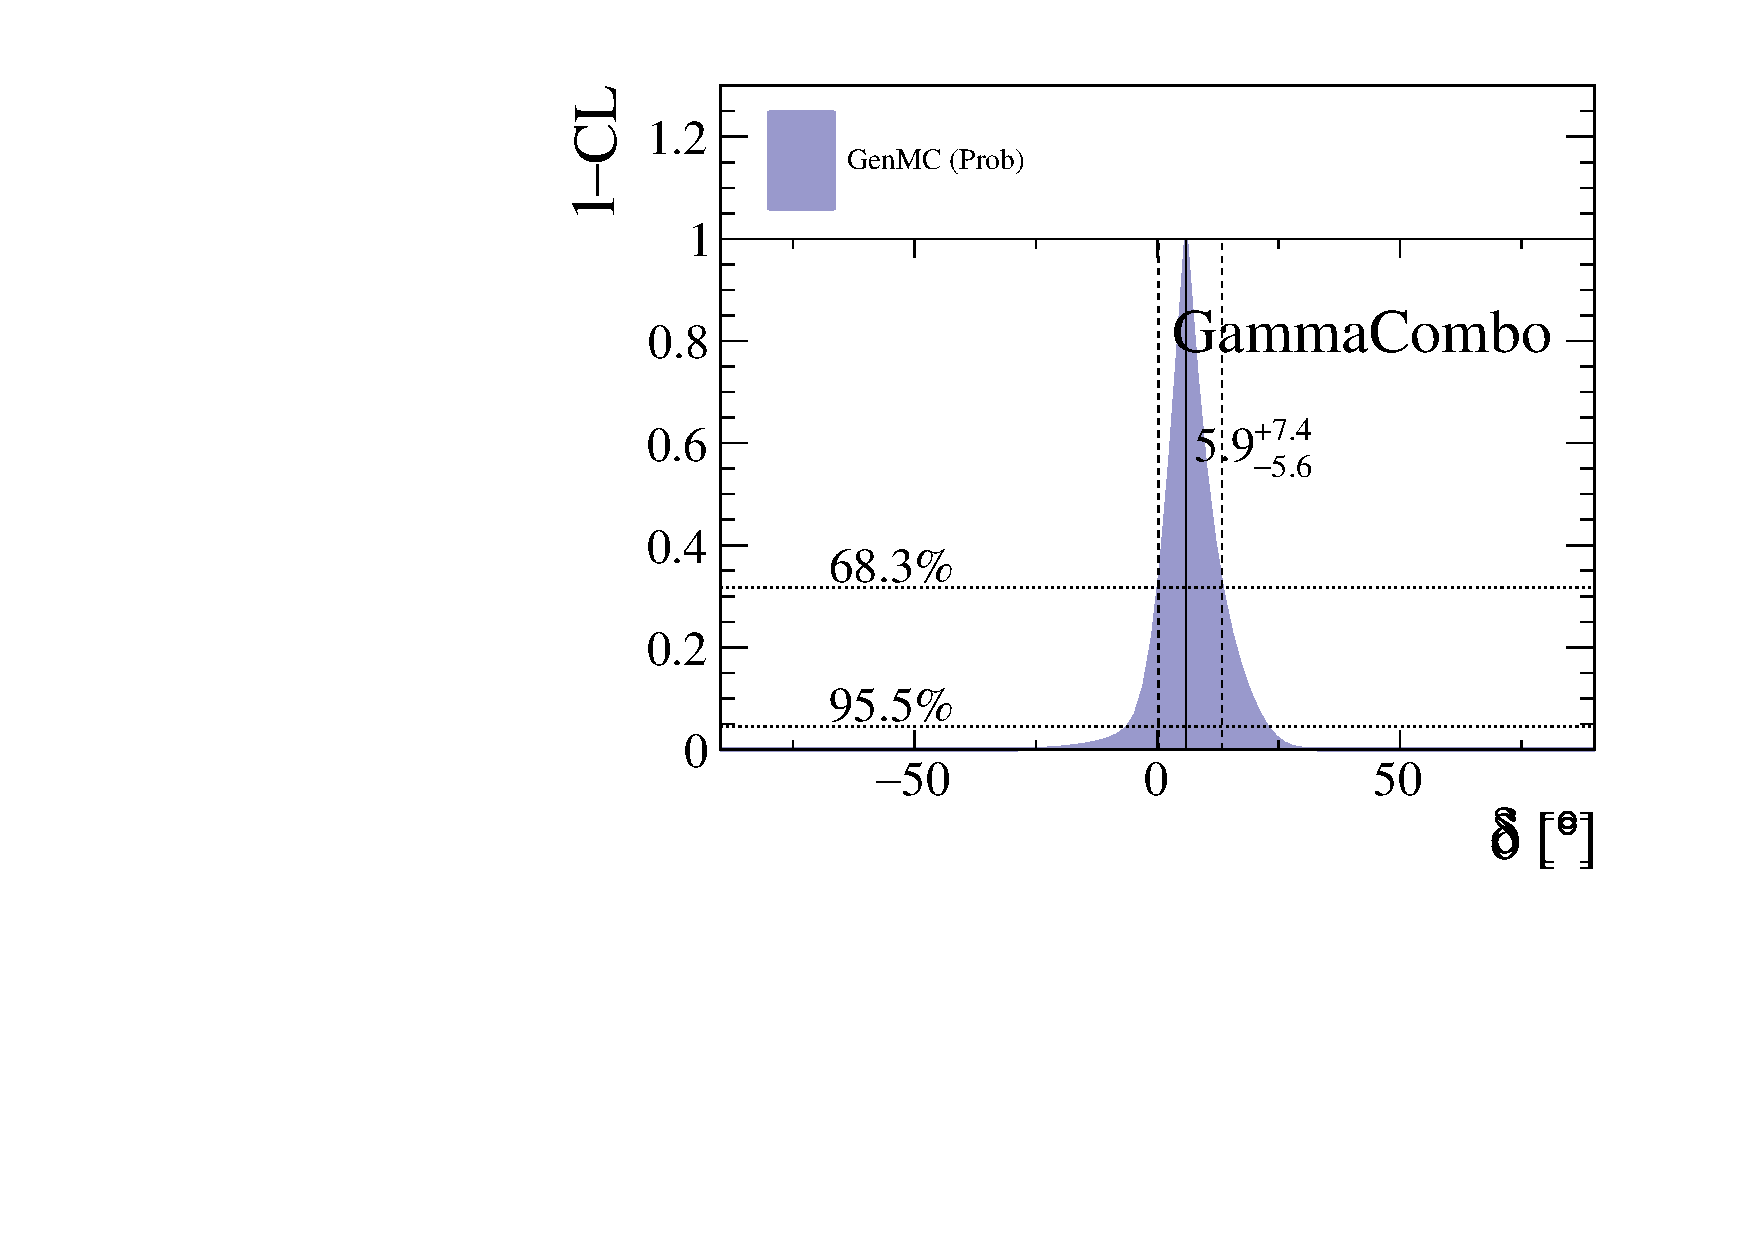
\includegraphics[width=0.4\textwidth, height = !]{figs/GammaCombo/signal_DsKpipi_CPV_MC/cartesian_cp_coeff_d.pdf} 
		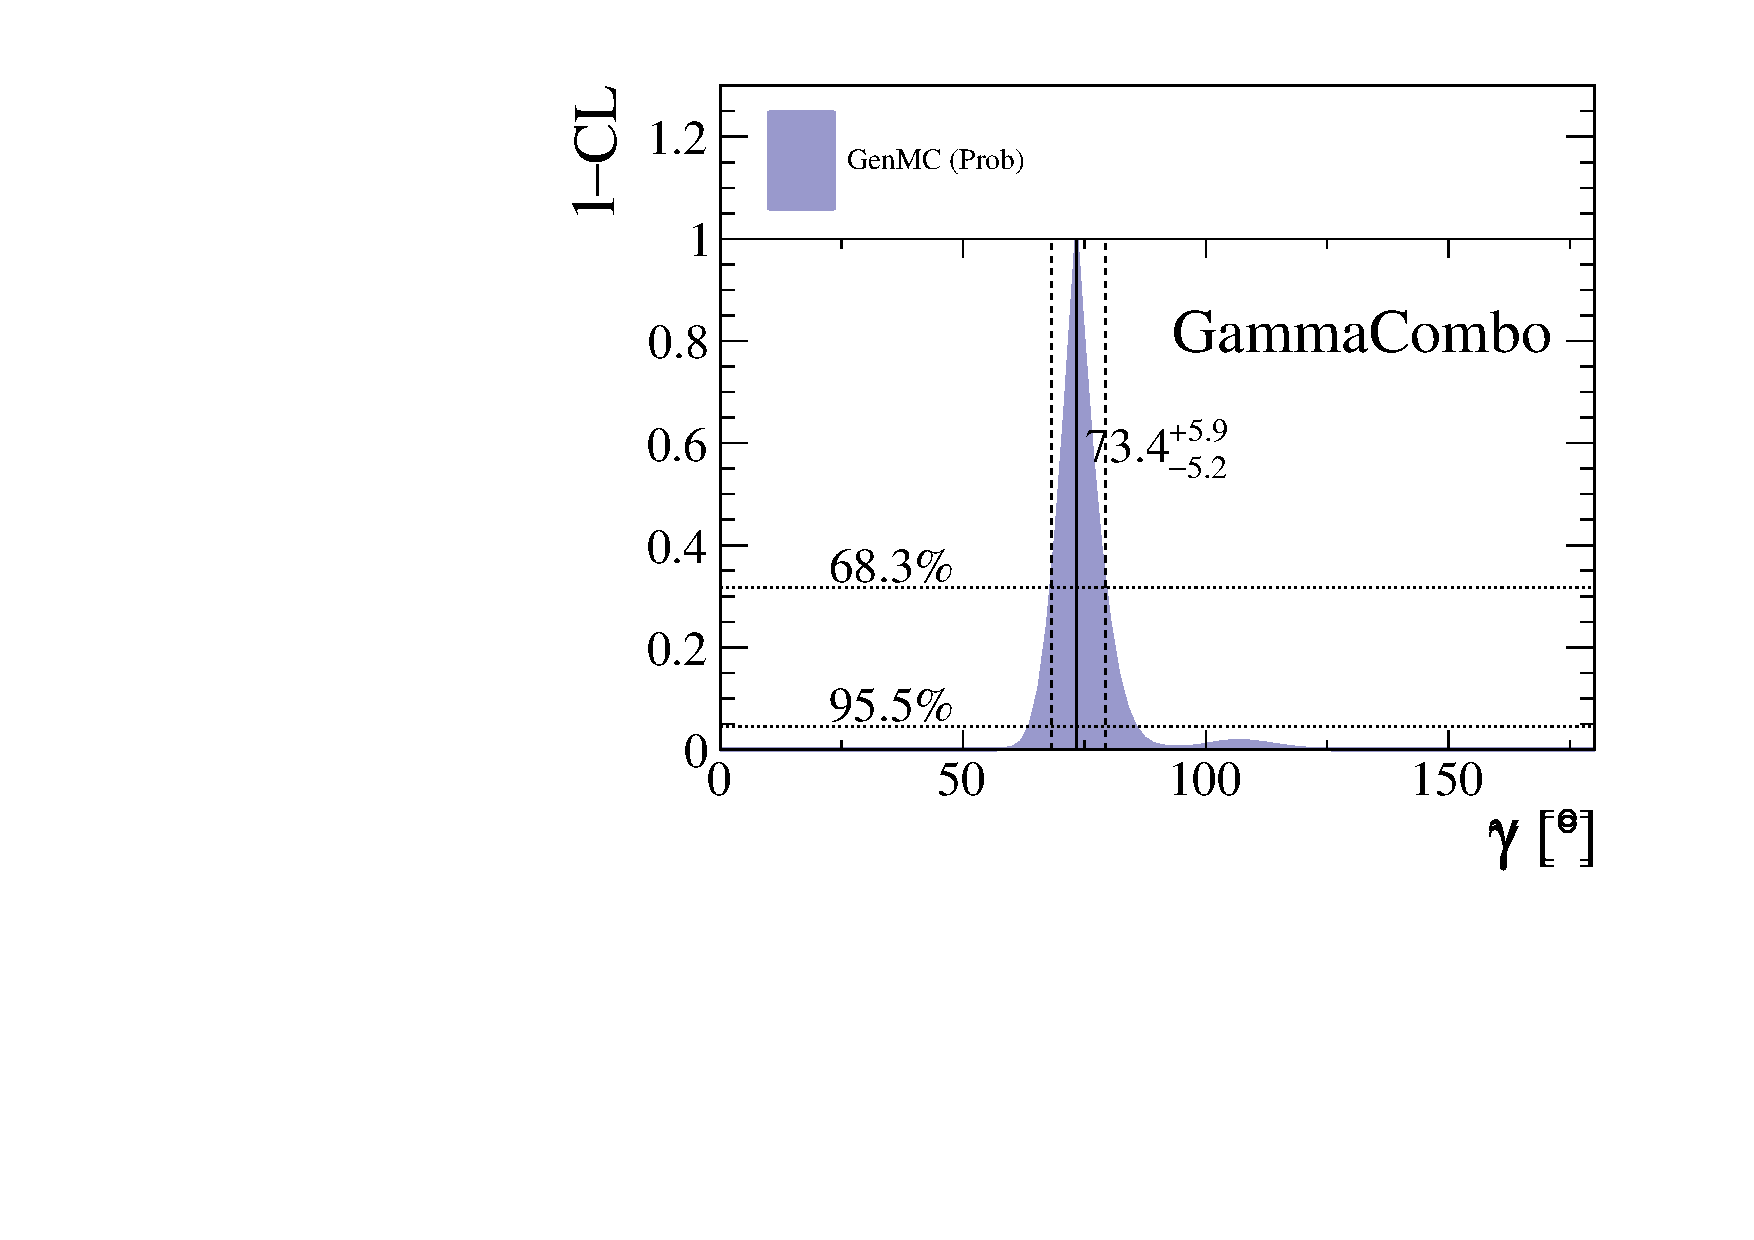
\includegraphics[width=0.4\textwidth, height = !]{figs/GammaCombo/signal_DsKpipi_CPV_MC/cartesian_cp_coeff_g.pdf} 
		\caption{The 1-CL contours for the physical observable $r,\kappa,\delta$ and $\gamma$ obtained with the phasespace-integrated fit to the \textsf{EVTGEN} toy sample. }
		\label{fig:FitGenCL}	
\end{figure} 

\begin{table}[h]
\caption{Result of the phasespace-integrated fit to \textsf{EVTGEN} toy events.} 		
%\resizebox{0.45\linewidth}{!}{
%  \scriptsize
  \centering
  \begin{tabular}
    {l c c c}
    \hline \hline
    & Generated &  Fit result  & Pull($\sigma$) \\   \hline
    $C$ & 0.759  &  $0.767 \pm 0.023 $  & 0.3         \\
    $D$ &  -0.314 &  $-0.194 \pm 0.205$ & 0.6         \\
    $\bar D$ &  -0.101 &  $-0.189 \pm 0.210$ & -0.4   \\
    $S$ &   -0.570 &  $-0.556 \pm 0.033$     & 0.4 \\
    $\bar S$ &  -0.643   &  $-0.683\pm 0.031$ & -1.3  \\
    \hline \hline
  \end{tabular}
    \label{tab:FitGenMC}
%    }
\end{table}

%\begin{table}[h]
%\caption{Result of the time-dependent amplitude fit to \textsf{EVTGEN} toy events.} 		
%%   \resizebox{0.45\linewidth}{!}{ 
%%  \scriptsize
%  \centering
%  \begin{tabular}
%    {l c c c}
%    \hline \hline
%    & Generated &  Fit result & Pull($\sigma$) \\   \hline
%    $x_-$ & 0.179  &  $0.135 \pm 0.050$ & -0.9	 \\
%    $y_-$ &  -0.324 & $-0.307 \pm 0.022$ 	& 0.8 \\
%    $x_+$ &  0.057 & $0.102 \pm 0.065$ & 0.6	 \\
%    $y_+$ &   0.366 &  $0.394 \pm 0.023$	& 1.3 \\
%    \hline \hline
%  \end{tabular}
%    \label{tab:FitGenMC2}
%%    }
%\end{table}

\begin{table}[h]
\caption{Results for the physical observables obtained from fits to \textsf{EVTGEN} toy events.} 		
%  \scriptsize
  \centering
  \begin{tabular}
    {l c c c c}
    \hline \hline
    & Generated &  Full PDF     &   Phasespace-integrated  \\   \hline
 $r$ & 0.370 & $0.372 \pm 0.015 $ & $0.372 \pm 0.015$  \\
 $\kappa$  &1.0 & 1.0 &  $1.000 \pm  0.035$  \\
 $\delta$ & $10.0^\circ$ &  $12.2 \pm  5.1$ & $12.3 \pm  5.1$   \\
 $\gamma$ & $71.1^\circ$ &   $73.2 \pm 5.5$ &  $73.4 \pm 5.5$\\
    \hline \hline
  \end{tabular}
      \label{tab:FitGenMC3}
\end{table}

      

%\begin{figure}[h]
%	\centering
%		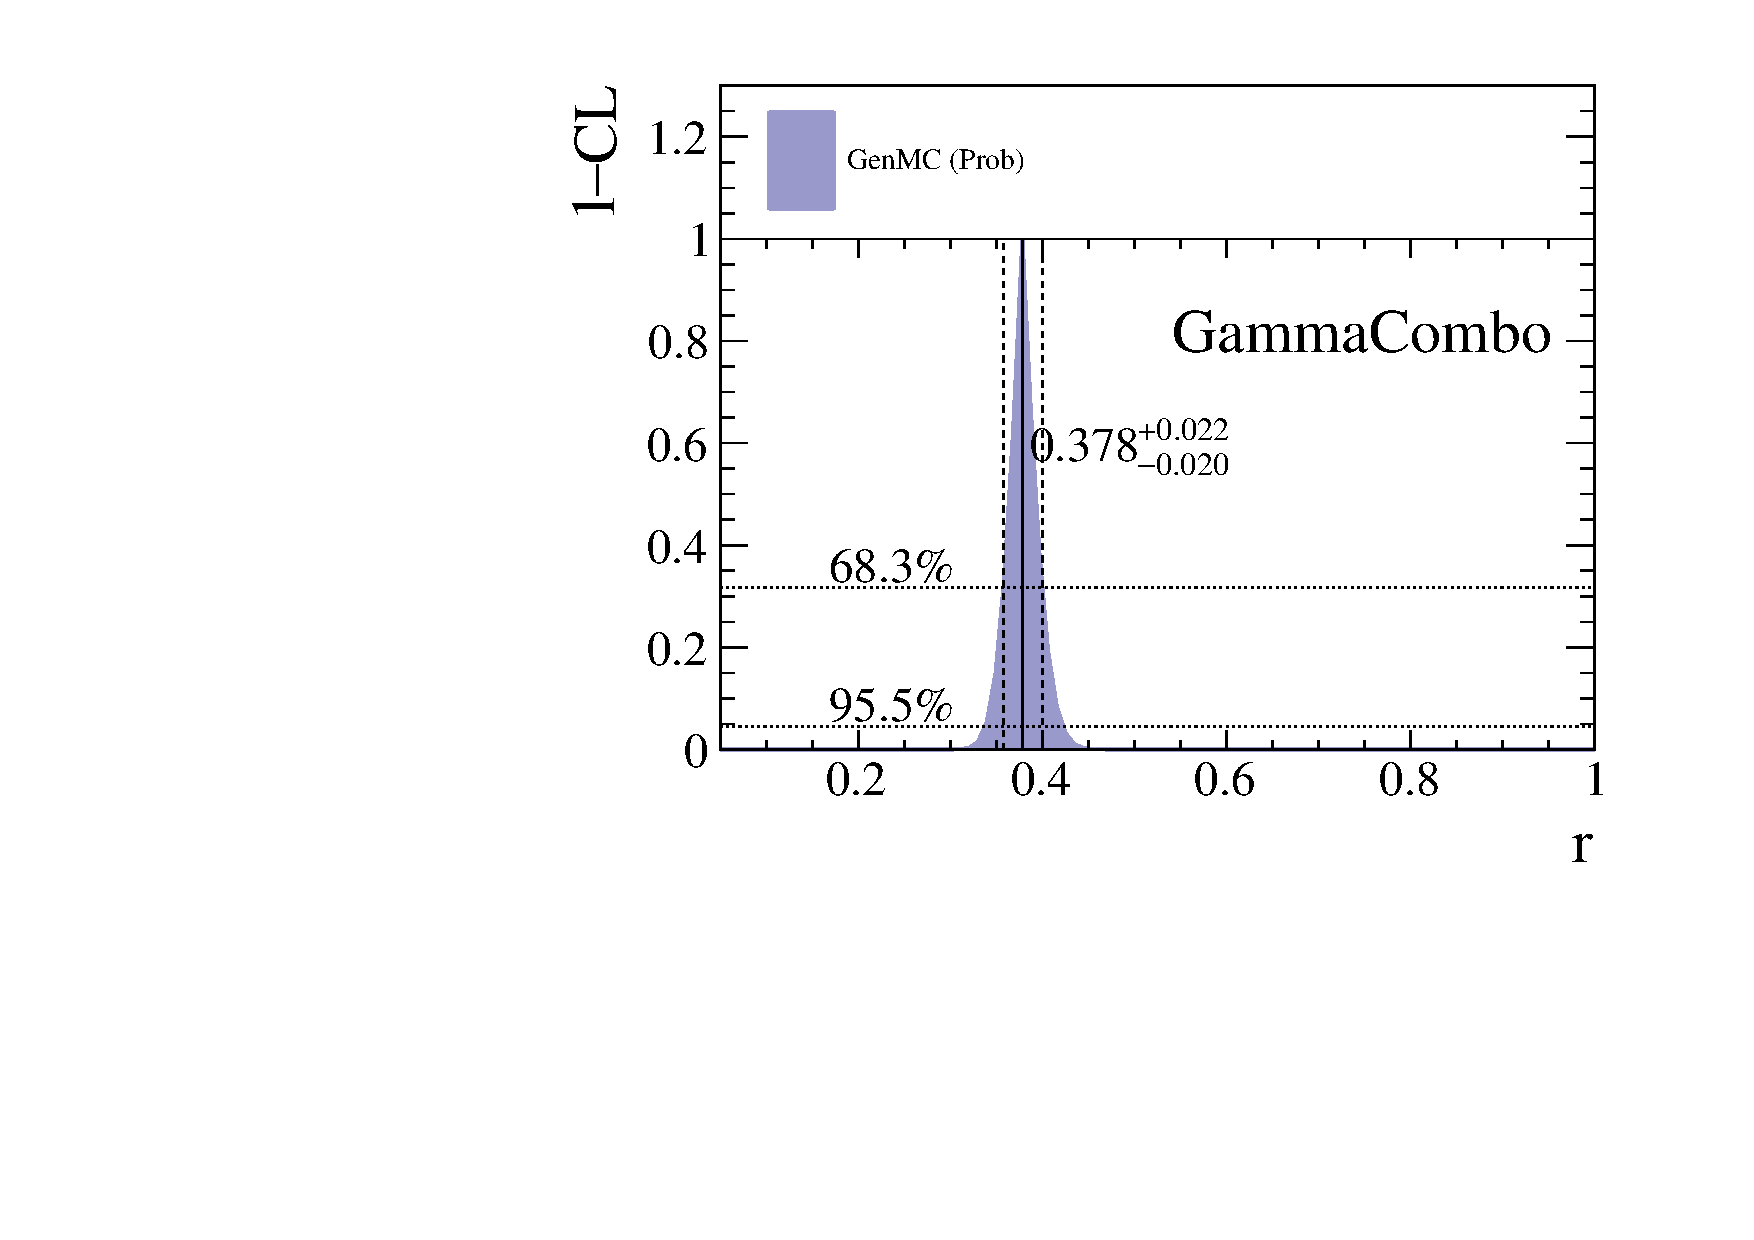
\includegraphics[width=0.4\textwidth, height = !]{figs/GammaCombo/signal_DsKpipi_CPV_MC/cartesian_GenMC_r.pdf} 		
%		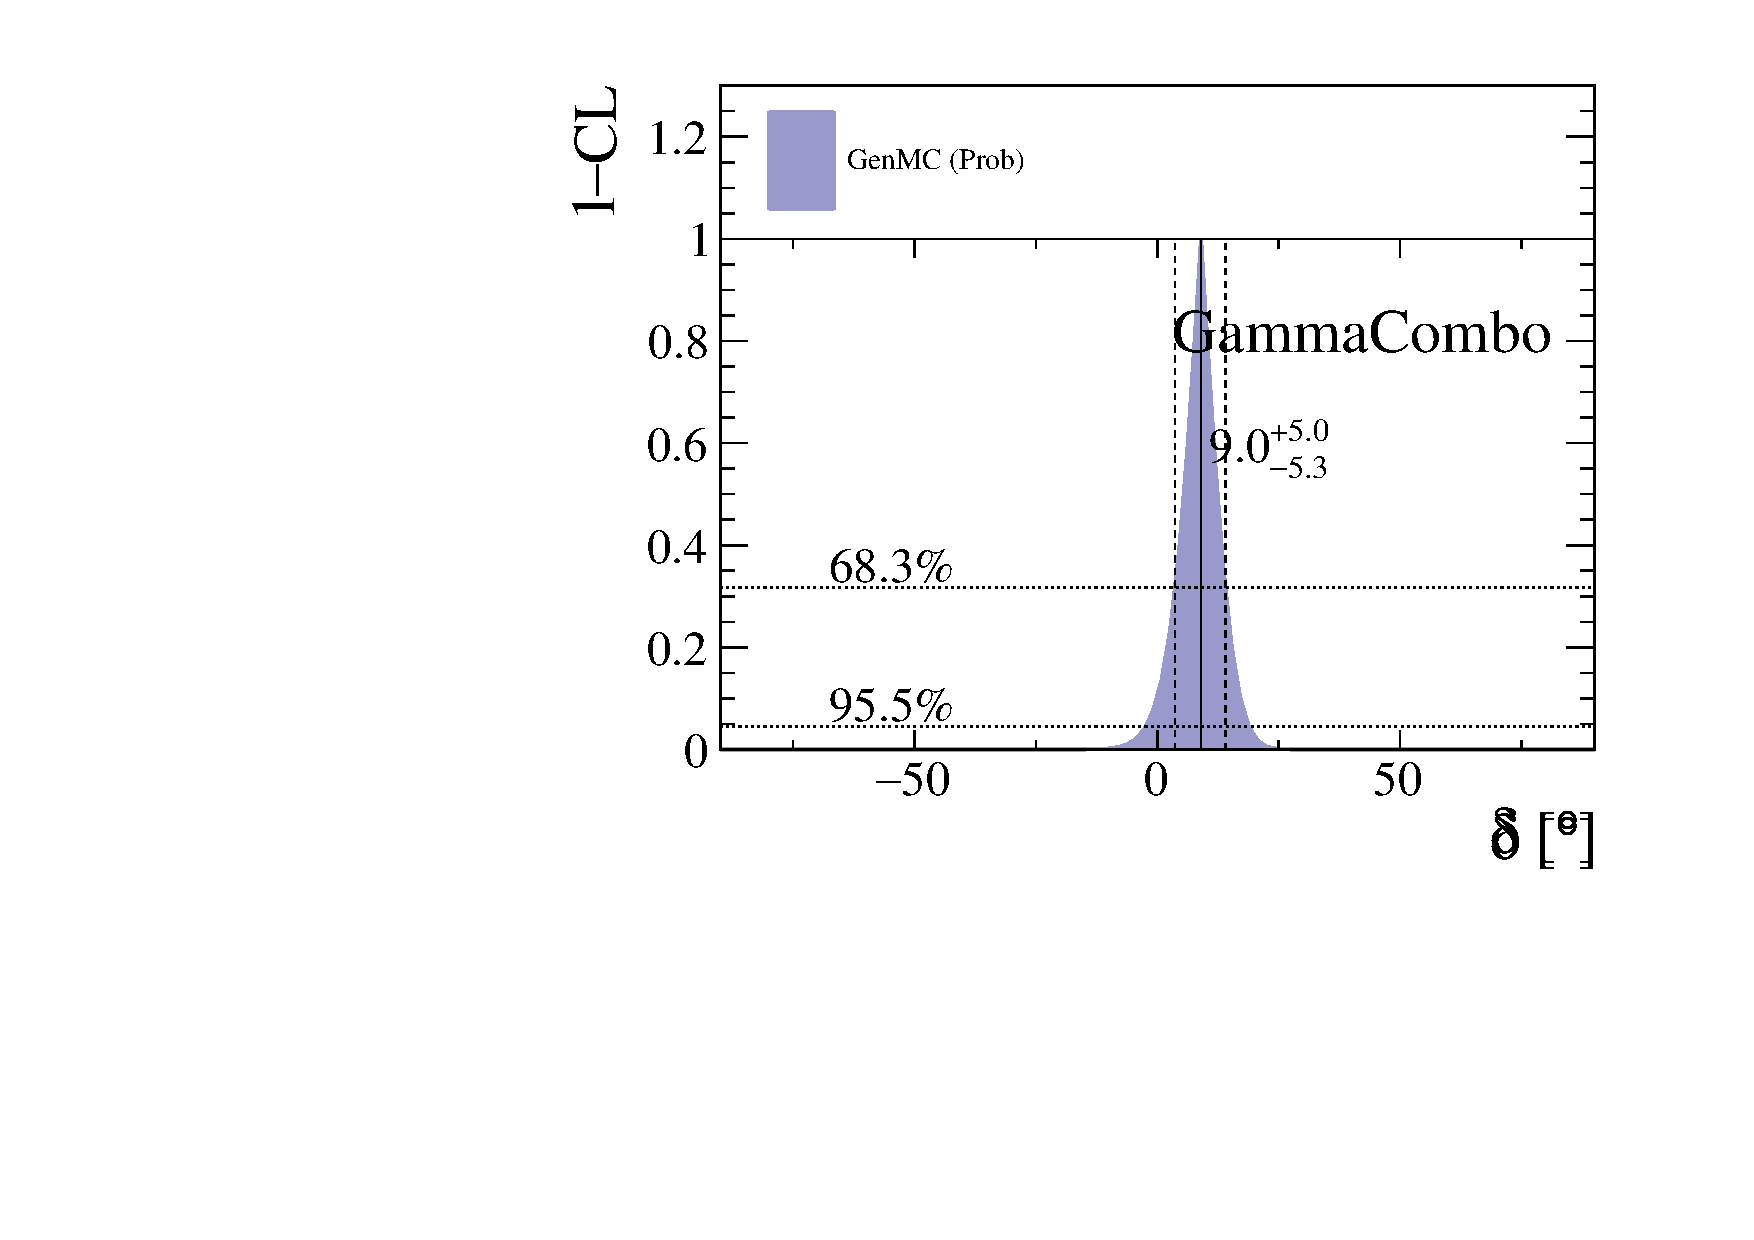
\includegraphics[width=0.4\textwidth, height = !]{figs/GammaCombo/signal_DsKpipi_CPV_MC/cartesian_GenMC_d.pdf} 
%		
%		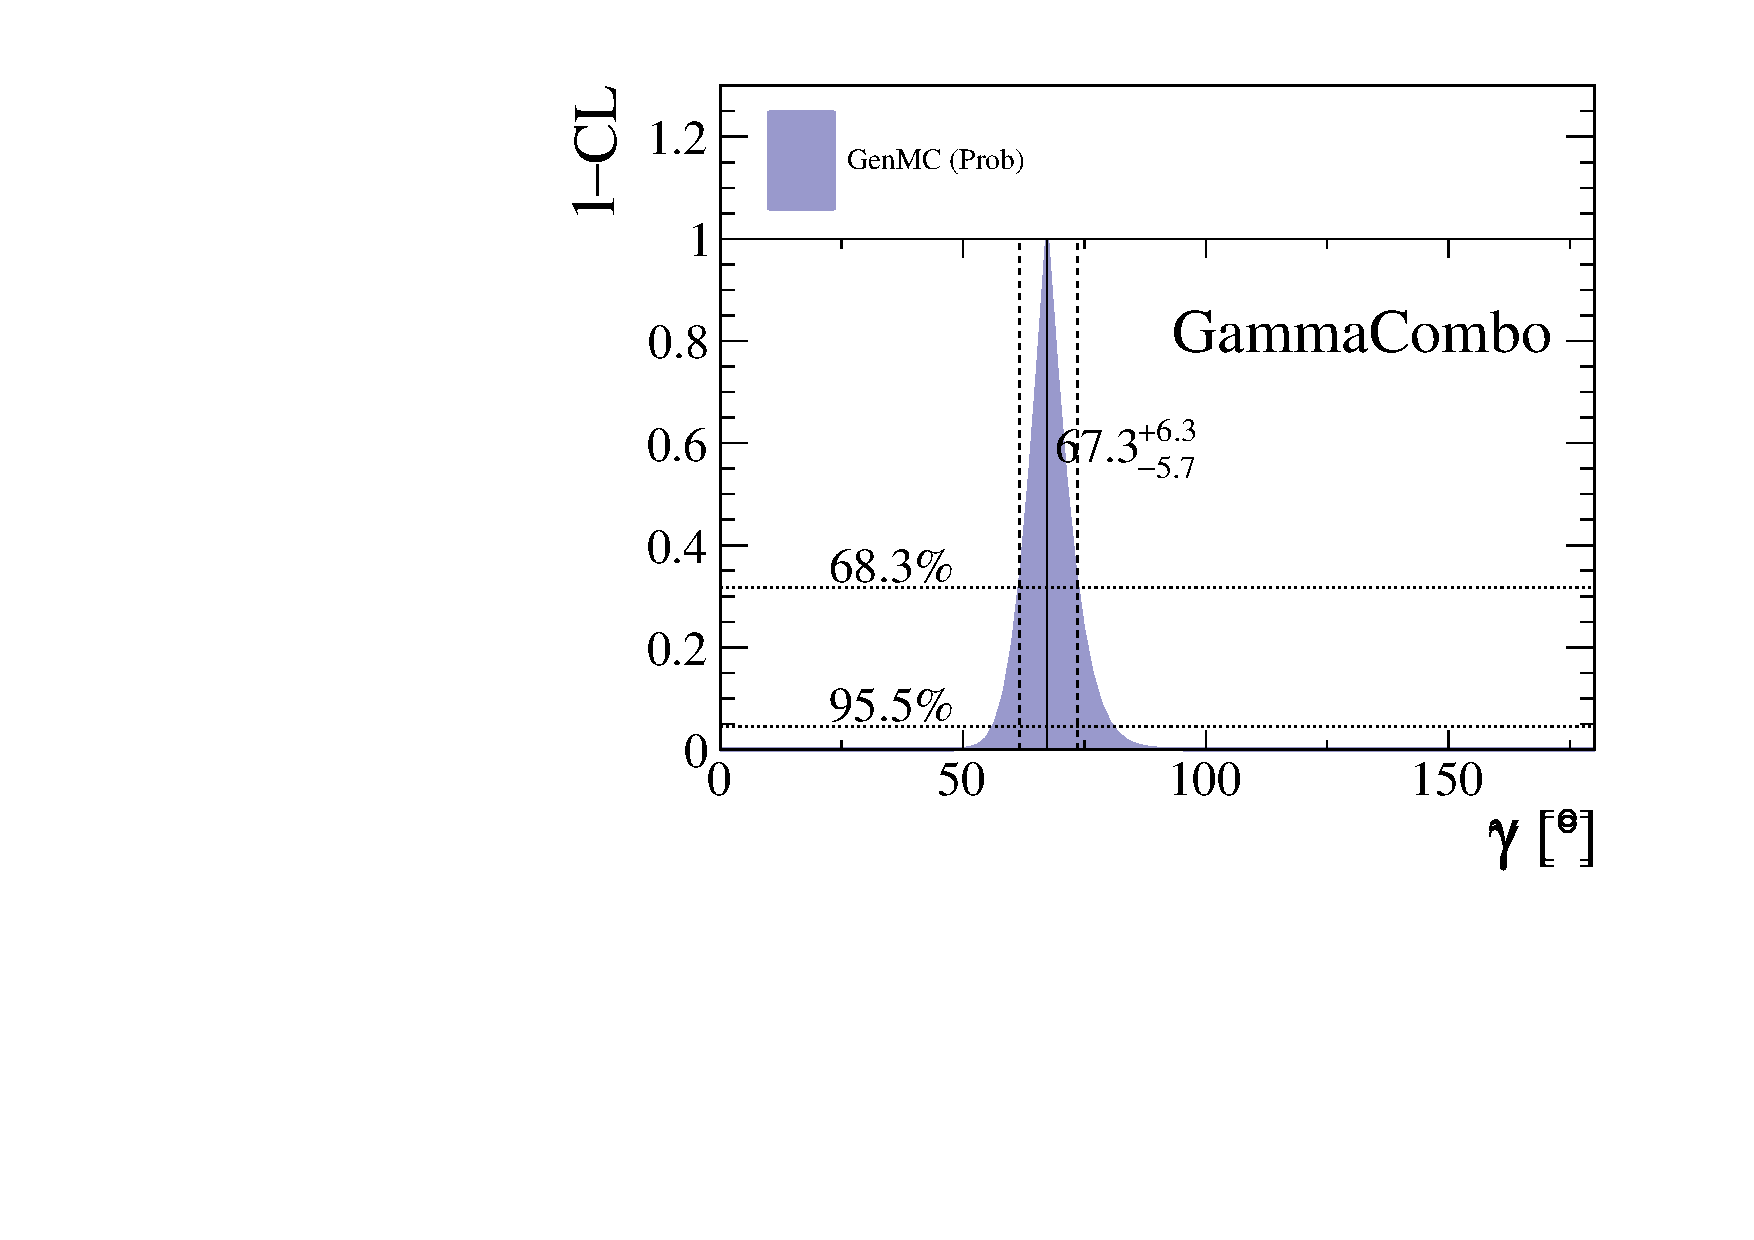
\includegraphics[width=0.4\textwidth, height = !]{figs/GammaCombo/signal_DsKpipi_CPV_MC/cartesian_GenMC_g.pdf} 
%		\caption{The 1-CL contours for the physical observable $r,\delta,\gamma$ obtained with the time-dependent amplitude fit fit to the \textsf{EVTGEN} toy sample. } 	
%\end{figure}  
    
